%%%%%%%%%%%%%%%%%%%%%%%%%%%%%%%%%%%%%%%%%%%%%%%%%%%%%%%%%%%%%%%%%%%%%%
%%%%%%%%%%%%%%%%%%%%%%%%%%%%%%%%%%%%%%%%%%%%%%%%%%%%%%%%%%%%%%%%%%%%%%
%%%%%%%%%%%%%%%%%%%%%%%%%%%%              SOFTWARE           %%%%%%%%%%%%%%%%%%%%%%%%%%%%
%%%%%%%%%%%%%%%%%%%%%%%%%%%%%%%%%%%%%%%%%%%%%%%%%%%%%%%%%%%%%%%%%%%%%%
%%%%%%%%%%%%%%%%%%%%%%%%%%%%%%%%%%%%%%%%%%%%%%%%%%%%%%%%%%%%%%%%%%%%%%
\section{Software}

The main analysis tasks (\texttt{C++} classes) used in the analysis are in the \texttt{PWGJE} and \texttt{PWGHF} library of the \texttt{AliPhysics} software package:
\begin{itemize}
\item \texttt{PWGHF/AliAnalysisTaskDmesonsFilterCJ} (filters D mesons and creates a set of particles with the D meson instead of the daughters);
\item \texttt{PWGHF/AliAnalysisTaskDJetCorrelations} (correlates each D meson found with a jet);
\item \texttt{PWGJE/EMCALJetTasks/AliEmcalJetTask} (finds and handles jets) ;%(what does this do?)
%\item \texttt{AliAnalysisTaskRhoSparse}. %(what does this do?)
\end{itemize}
The \texttt{AliRoot} version used for this analysis is the tag: \texttt{VO\_ALICE@AliPhysics::vAN-20200611\_ROOT6-1}.

The task used for this analysis generates a multiple axis histogram (\texttt{THnSparse}) that keeps information about: \zpar, jet \pt, D-meson \pt\ and D-meson invariant mass.

The post-processing includes: projection of the \texttt{THnSparse} onto lower-dimensional histograms, raw signal extraction, response matrix generation, B feed-down correction, unfolding and the final plotting.
The post-processing is relatively light-weight and is performed directly in a personal computer. This code is written using the \texttt{C++} with \texttt{ROOT} coupled with \texttt{Python} and \texttt{Bash}.

The analysis follows closely the analysis procedure of the \Dzero-jet \pt\ differential cross-section measurement in \pPb\ collisions at \snn=5.02~TeV: https://aliceinfo.cern.ch/Notes/node/784 and in \pp\ collisions at \s=5.02~TeV: https://aliceinfo.cern.ch/Notes/node/840.

%%%%%%%%%%%%%%%%%%%%%%%%%%%%%%%%%%%%%%%%%%%%%%%%%%%%%%%%%%%%%%%%%%%%%%
%%%%%%%%%%%%%%%%%%%%%%%%%%%%%%%%%%%%%%%%%%%%%%%%%%%%%%%%%%%%%%%%%%%%%%
%%%%%%%%%%%%%%%%%%%%%%%%%%%%              DATASETS            %%%%%%%%%%%%%%%%%%%%%%%%%%%%
%%%%%%%%%%%%%%%%%%%%%%%%%%%%%%%%%%%%%%%%%%%%%%%%%%%%%%%%%%%%%%%%%%%%%%
%%%%%%%%%%%%%%%%%%%%%%%%%%%%%%%%%%%%%%%%%%%%%%%%%%%%%%%%%%%%%%%%%%%%%%

\section{Dataset and Event Selection}

For this analysis we use the data collected by ALICE in 2017 during the Minimum Bias period of the \pp\ collisions at $\s=5.02$~TeV. This data corresponds to the following data taking periods:
LHC17p and LHC17q pass1, FAST and CENT\_woSDD productions were merged.
The complete list of runs used in this analysis are:

LHC17p\_CENT\_woSDD: 282343, 282342, 282341, 282340, 282314, 282313, 282312, 282309, 282307, 282306, 282305, 282304, 282303, 282302, 282247, 282230, 282229, 282227, 282224, 282206, 282189, 282147, 282146, 282127, 282126, 282125, 282123, 282122, 282120, 282119, 282118, 282099, 282098, 282078, 282051, 282050, 282031, 282030, 282025, 282021, 282016, 282008 \\
LHC17p\_FAST: 282343, 282342, 282341, 282340, 282314, 282313, 282312, 282309, 282307, 282306, 282305, 282304, 282303, 282302, 282247, 282230, 282229, 282227, 282224, 282206, 282189, 282147, 282146, 282127, 282126, 282125, 282123, 282122, 282120, 282119, 282118, 282099, 282098, 282078, 282051, 282050, 282031, 282025, 282021, 282016, 282008 \\
LHC17q\_CENT\_woSDD: 282367, 282366, 282365 \\
LHC17q\_FAST: 282367, 282366, 282365

Events were selected using the event selection \texttt{kINT7}. Note that the analysis is performed in \texttt{AOD}, where the beam-gas and gas-gas events have been filtered out.
Events were further filtered using the Physics Selection, and selection provided by:
\begin{itemize}
\item \texttt{AliAnalysisTaskEmcal::IsEventSelected()}, which rejects events based on event vertex quality, in particular requiring a reconstructed vertex position not farther than 10 cm from the center of the detector along the beam axis; and a distance between the SPD vertex and the V0 vertex not larger than 0.5 cm;
%\item \texttt{AliRDHFCutsDStartoKpipi::IsEventSelected(AliVEvent*)}, which rejects events for D$^*$ candidates based on event vertex quality and pileup
\item \texttt{AliRDHFCutsD0toKpi::IsEventSelected(AliVEvent*)}, which rejects events for D$^0$ candidates based on event vertex quality and pileup.
\end{itemize}

The total number of events is about 900  M  out of  analysed (after all the selections outlined below).
Results shown in this {\it note} come from the LEGO trains 
\begin{itemize}
\item HFCJ\_pp 744, 757, 745, 751 (standard and 4 other cuts)
\end{itemize}
 for R=0.2, 0.3, 0.4 and 0.6 respectively.
% (including: LHC17p\_pass1\_FAST, LHC17p\_pass1\_CENT\_woSDD, LHC17q\_pass1\_FAST, LHC17q\_pass1\_CENT\_woSDD).
The pp dataset is Correl\_LHC17pq. 
\subsection{Monte Carlo productions}

For this analysis the Monte Carlo production LHC18a4a2\_g3\_fast was used, anchored to the 2017 \pp\ data taking periods LHC17p and LHC17q and the FAST production. The FAST production simulation is used to correct the data sample, which is the merged: FAST+CENT\_woSDD, assuming that efficiencies and detector response are the same for both.
The simulations uses PYTHIA6 with the Perugia2011 tune as particle generator at $\s=5.02$~TeV.
The charm content has been enhanced by requesting a \ccbar\ in 50\% of the events and a \bbbar\ in the remaining half.
Furthermore, all D mesons are forced to decay hadronically.
This MC production is used to compute the D-meson efficiency with jets, acceptance corrections and a response matrix of D-tagged jets with prompt and non-prompt \Dzero\ : c,~b~$\rightarrow$ ~\Dzero\ .

Results shown in this {\it note} come from the LEGO trains 
\begin{itemize}
\item HFCJ\_ppMC 1059, 1071, 1061, 1062 (standard and 4 other cuts)
\item HFCJ\_ppMC 1060, 1078, 722, 721 (JES)
\end{itemize}
 for R=0.2, 0.3, 0.4 and 0.6 respectively.
%%%%%%%%%%%%%%%%%%%%%%%%%%%%%%%%%%%%%%%%%%%%%%%%%%%%%%%%%%%%%%%%%%%%%%
%%%%%%%%%%%%%%%%%%%%%%%%%%%%%%%%%%%%%%%%%%%%%%%%%%%%%%%%%%%%%%%%%%%%%%
%%%%%%%%%%%%%%%%%%%%%%%%%%%%    D-MESON SELECTION   %%%%%%%%%%%%%%%%%%%%%%%%%%%%
%%%%%%%%%%%%%%%%%%%%%%%%%%%%%%%%%%%%%%%%%%%%%%%%%%%%%%%%%%%%%%%%%%%%%%
%%%%%%%%%%%%%%%%%%%%%%%%%%%%%%%%%%%%%%%%%%%%%%%%%%%%%%%%%%%%%%%%%%%%%%

\section{D-Meson Selection}
\label{sec:DmesonSel}

The D mesons were reconstructed through their hadronic decay channels~\cite{Tanabashi:2018oca}:
\begin{eqnarray*}
\Dzero (\bar{\Dzero}) &\to& {\rm K}^{\mp} + \pi^{\pm}  , {\text{ BR}} = 3.89\pm {0.04} \%\\
\end{eqnarray*}
The selection strategy is based on the topological displacement of the secondary vertex from the primary vertex due to their relatively large lifetime.

The candidate vertices are read from the \texttt{AOD} friend chain \texttt{AliAOD.VertexingHF.root}. A list of topological and kinematic cuts applied for \Dzero\ in \pp\ collisions at $\s=5.02$~TeV.
The same quality track selection on the decay products used for the D-meson spectra analysis of the same datasets has been used in this analysis.
For the final jet spectrum we will apply $\ptd> 2, 3$~\GeVc\ on the D mesons. The accepted $|y_{\rm D}|$ range is \pt-dependent, with the upper limit growing from $0.5$ to $0.8$ at $\pt=5$~\GeVc.

\begin{table}[bth]
\caption{\Dzero\ cuts for \pp\ collisions at $\s=5.02$~TeV. Default set.}
\label{DZeroCutsppC0}
\resizebox{\textwidth}{!}{%
\begin{tabular}{lrrrrrrrrrrrrr}
        \hline
    $p_{\mathrm T,\Dzero}$ (\GeVc) 	&$0.5-1$	& $1-2$	& $2-3$	& $3-4$	& $4-5$	& $5-6$	& $6-7$	& $7-8$	& $8-10$& $10-12$	& $12-16$	& $16-24$	& $24-36$ \\ \hline
    $\Delta M_{\Dzero} (\GeVcsq)$		& 0.4 	& 0.4	& 0.4	& 0.4	& 0.4	& 0.4	& 0.4	& 0.4	& 0.4	& 0.4		& 0.4		& 0.4		& 0.4 \\ \hline
    DCA (cm)						& 0.03	& 0.03	& 0.03	& 0.03	& 0.03	& 0.03	& 0.03	& 0.03	& 0.03	& 0.03		& 0.03		& 0.03		& 0.03 \\ \hline
    $\cos(\theta^{*})$				& 0.8	& 0.8	& 0.8	& 0.8	& 0.8	& 0.8	& 0.8	& 0.8	& 0.9	& 0.9		& 1			& 1			& 1\\ \hline
    $p_{\mathrm T,K}$ (\GeVc)		& 0.5	& 0.5	& 0.7	& 0.7	& 0.7	& 0.7	& 0.7	& 0.7	& 0.7	& 0.7		& 0.7		& 0.7		& 0.7 \\ \hline
    $p_{\mathrm T,\pi}$ (\GeVc) 		& 0.5	& 0.5	& 0.7	& 0.7	& 0.7	& 0.7	& 0.7	& 0.7	& 0.7	& 0.7		& 0.7		& 0.7		& 0.7 \\ \hline
    $d_{0}^{K}$  (cm) 				& 0.1	& 0.1 	& 0.1 	& 0.1 	& 0.1 	& 0.1 	& 0.1 	& 0.1 	& 0.1 	& 0.1 		& 0.1 		& 0.1 		& 0.1 \\ \hline
    $d_{0}^{\pi}$  (cm) 				& 0.1	& 0.1 	& 0.1 	& 0.1 	& 0.1 	& 0.1 	& 0.1 	& 0.1 	& 0.1 	& 0.1 		& 0.1 		& 0.1 		& 0.1 \\ \hline
    $d_{0}^{K}\cdot d_{0}^{\pi}$ $(10^{-4}{\rm cm}^2)$
								& -5 		& -3.5 	& -3 		& -3 		& -1.5 	& -1 		& -0.8 	& -0.8 	& -0.5 	& -0.5 		& 1 			& 1			& 1   \\ \hline
    $\cos(\theta_{\rm point})$ 		& 0.95	& 0.95	& 0.95	& 0.95	& 0.95	& 0.95	& 0.95	& 0.95	& 0.95	& 0.95		& 0.95		& 0.90 		& 0.90 \\ \hline
%    $\cos(\theta_{{\rm point},xy})$ 		& 0	& 0	& 0	& 0	& 0	& 0	& 0	& 0	& 0	& 0		& 0		& 0 		& 0 \\ \hline
    $L_{xy}/\sigma_{L_{xy}} ({\rm cm})$	& 5 		& 5 		& 5 		& 5 		& 5 		& 4 		& 4 		& 4 		& 3 		& 3 			& 3 			& 3 			& 3 \\ \hline
\end{tabular}
}
\end{table}


    
\begin{table}[bth]
\caption{\Dzero\ cuts for \pp\ collisions at $\s=5.02$~TeV. Cuts 1}
\label{DZeroCutsppC1}
\resizebox{\textwidth}{!}{%
\begin{tabular}{lrrrrrrrrrrrrr}
    \hline
    $p_{\mathrm T,\Dzero}$ (\GeVc) 	&$0.5-1$	& $1-2$	& $2-3$	& $3-4$	& $4-5$	& $5-6$	& $6-7$	& $7-8$	& $8-10$& $10-12$	& $12-16$	& $16-24$	& $24-36$ \\ \hline
    $\Delta M_{\Dzero} (\GeVcsq)$		& 0.005 	& 0.005	& 0.4	& 0.4	& 0.4	& 0.4	& 0.4	& 0.4	& 0.4	& 0.4		& 0.4		& 0.4		& 0.4 \\ \hline
    DCA (cm)						& 0.01	& 0.01	& 0.03	& 0.03	& 0.03	& 0.03	& 0.03	& 0.03	& 0.03	& 0.03		& 0.03		& 0.03		& 0.03 \\ \hline
%    $\cos(\theta^{*})$				& 0.8	& 0.8	& 0.8	& 0.8	& 0.8	& 0.8	& 0.8	& 0.8	& 0.9	& 0.9		& 1			& 1			& 1\\ \hline
%    $p_{\mathrm T,K}$ (\GeVc)		& 0.5	& 0.5	& 0.7	& 0.7	& 0.7	& 0.7	& 0.7	& 0.7	& 0.7	& 0.7		& 0.7		& 0.7		& 0.7 \\ \hline
%    $p_{\mathrm T,\pi}$ (\GeVc) 		& 0.5	& 0.5	& 0.7	& 0.7	& 0.7	& 0.7	& 0.7	& 0.7	& 0.7	& 0.7		& 0.7		& 0.7		& 0.7 \\ \hline
%    $d_{0}^{K}$  (cm) 				& 0.1	& 0.1 	& 0.1 	& 0.1 	& 0.1 	& 0.1 	& 0.1 	& 0.1 	& 0.1 	& 0.1 		& 0.1 		& 0.1 		& 0.1 \\ \hline
%    $d_{0}^{\pi}$  (cm) 				& 0.1	& 0.1 	& 0.1 	& 0.1 	& 0.1 	& 0.1 	& 0.1 	& 0.1 	& 0.1 	& 0.1 		& 0.1 		& 0.1 		& 0.1 \\ \hline
    $d_{0}^{K}\cdot d_{0}^{\pi}$ $(10^{-4}{\rm cm}^2)$
								& -6 		& -6.5 	& -2.7 	& -2.7 	& -1.3 	& -0.9 	& -0.8 	& -0.7 	& -0.5 	& -0.5 		& 1 			& 99.99		& 99.99   \\ \hline
    $\cos(\theta_{\rm point})$ 		& 0.93	& 0.93	& 0.93	& 0.93	& 0.93	& 0.93	& 0.93	& 0.93	& 0.93	& 0.93		& 0.93		& 0.87 		& 0.87	 \\ \hline
%    $\cos(\theta_{{\rm point},xy})$ 		& 0	& 0	& 0	& 0	& 0	& 0	& 0	& 0	& 0	& 0		& 0		& 0 		& 0 \\ \hline
    $L_{xy}/\sigma_{L_{xy}} ({\rm cm})$	& 4 		& 4 		& 4 		& 4 		& 4 		& 3 		& 3		& 3 		& 2 		& 2 			& 2 			& 2 			& 2 \\ \hline
    \end{tabular}
}\end{table}

\begin{table}[bth]

\caption{\Dzero\ cuts for \pp\ collisions at $\s=5.02$~TeV. Cuts 2}
\label{DZeroCutsppC2}
\resizebox{\textwidth}{!}{%
\begin{tabular}{lrrrrrrrrrrrrr}
    \hline
    $p_{\mathrm T,\Dzero}$ (\GeVc) 	&$0.5-1$	& $1-2$	& $2-3$	& $3-4$	& $4-5$	& $5-6$	& $6-7$	& $7-8$	& $8-10$& $10-12$	& $12-16$	& $16-24$	& $24-36$ \\ \hline
    $\Delta M_{\Dzero} (\GeVcsq)$		& 0.005 	& 0.005   & 0.4		& 0.4	& 0.4	& 0.4	& 0.4	& 0.4	& 0.4	& 0.4		& 0.4		& 0.4		& 0.4 \\ \hline
    DCA (cm)						& 0.01	& 0.01	& 0.03	& 0.03	& 0.03	& 0.03	& 0.03	& 0.03	& 0.03	& 0.03		& 0.03		& 0.03		& 0.03 \\ \hline
    
    %$\cos(\theta^{*})$				& 0.8	& 0.8	& 0.8	& 0.8	& 0.8	& 0.8	& 0.8	& 0.8	& 0.9	& 0.9		& 1			& 1			& 1\\ \hline
    %$p_{\mathrm T,K}$ (\GeVc)		& 0.5	& 0.5	& 0.7	& 0.7	& 0.7	& 0.7	& 0.7	& 0.7	& 0.7	& 0.7		& 0.7		& 0.7		& 0.7 \\ \hline
    %$p_{\mathrm T,\pi}$ (\GeVc) 		& 0.5	& 0.5	& 0.7	& 0.7	& 0.7	& 0.7	& 0.7	& 0.7	& 0.7	& 0.7		& 0.7		& 0.7		& 0.7 \\ \hline    
    %$d_{0}^{K}$  (cm) 				& 0.1	& 0.1 	& 0.1 	& 0.1 	& 0.1 	& 0.1 	& 0.1 	& 0.1 	& 0.1 	& 0.1 		& 0.1 		& 0.1 		& 0.1 \\ \hline
    %$d_{0}^{\pi}$  (cm) 				& 0.1	& 0.1 	& 0.1 	& 0.1 	& 0.1 	& 0.1 	& 0.1 	& 0.1 	& 0.1 	& 0.1 		& 0.1 		& 0.1 		& 0.1 \\ \hline
    $d_{0}^{K}\cdot d_{0}^{\pi}$ $(10^{-4}{\rm cm}^2)$
								& -6 		& -6.5 	& -2.2 	& -2 		& -1 		& -0.8 	& -0.7 	& -0.6 	& -0.4 	& -0.4 		& 1 			& 99.99		& 99.99   \\ \hline
    $\cos(\theta_{\rm point})$ 		& 0.95	& 0.95	& 0.90	& 0.90	& 0.90	& 0.90	& 0.90	& 0.90	& 0.90	& 0.90		& 0.90		& 0.85 		& 0.85 \\ \hline
%    $\cos(\theta_{{\rm point},xy})$ 		& 0	& 0	& 0	& 0	& 0	& 0	& 0	& 0	& 0	& 0		& 0		& 0 		& 0 \\ \hline
    $L_{xy}/\sigma_{L_{xy}} ({\rm cm})$	& 3 		& 3 		& 3 		& 3 		& 3 		& 2 		& 2 		& 2 		& 1 		& 1 			& 1 			& 1 			& 1 \\ \hline
    \end{tabular}
}    \end{table}

\begin{table}[bth]
\caption{\Dzero\ cuts for \pp\ collisions at $\s=5.02$~TeV. Cuts 3}
\label{DZeroCutsppC3}
\resizebox{\textwidth}{!}{%
\begin{tabular}{lrrrrrrrrrrrrr}
    \hline
    $p_{\mathrm T,\Dzero}$ (\GeVc) 	&$0.5-1$	& $1-2$	& $2-3$	& $3-4$	& $4-5$	& $5-6$	& $6-7$	& $7-8$	& $8-10$	& $10-12$	& $12-16$	& $16-24$	& $24-36$ \\ \hline
    $\Delta M_{\Dzero} (\GeVcsq)$		&0.005	&0.005	&0.4		&0.4		&0.4		&0.4		&0.4		&0.4		&0.4		&0.4			&0.4		&0.4		&0.4	 \\ \hline
   DCA (cm)						&0.01	&0.01	&0.03	&0.03	&0.03	&0.03	&0.03	&0.03	&0.03	&0.03		&0.03	&0.03	&0.03	 \\ \hline
%    $\cos(\theta^{*})$				&0.8		&0.8		&0.8		&0.8		&0.8		&0.8		&0.8		&0.8		&0.9		&0.9			&1		&1		&1	 \\ \hline
%    $p_{\mathrm T,K}$ (\GeVc)		&0.5		&0.5		&0.7		&0.7		&0.7		&0.7		&0.7		&0.7		&0.7		&0.7			&0.7		&0.7		&0.7	 \\ \hline
%    $p_{\mathrm T,\pi}$ (\GeVc)		&0.5		&0.5		&0.7		&0.7		&0.7		&0.7		&0.7		&0.7		&0.7		&0.7			&0.7		&0.7		&0.7	 \\ \hline
%    $d_{0}^{K}$  (cm)				&0.1		&0.1		&0.1		&0.1		&0.1		&0.1		&0.1		&0.1		&0.1		&0.1			&0.1		&0.1		&0.1	 \\ \hline
%    $d_{0}^{\pi}$  (cm)				&0.1		&0.1		&0.1		&0.1		&0.1		&0.1		&0.1		&0.1		&0.1		&0.1			&0.1		&0.1		&0.1	 \\ \hline
    $d_{0}^{K}\cdot d_{0}^{\pi}$ $(10^{-4}{\rm cm}^2)$ 
    								&-6		&-6.5	&-2		&-1.2	&-0.8	&-0.8	&-0.8	&-0.7	&-0.5	&-0.5		&0.1		&99.99	&99.99	 \\ \hline
    $\cos(\theta_{\rm point})$		&0.95	&0.95	&0.8		&0.8		&0.85	&0.85	&0.85	&0.85	&0.85	&0.85		&0.85	&0.85	&0.85 \\ \hline
%    $\cos(\theta_{{\rm point},xy})$&0	&0	&0	&0	&0	&0	&0	&0	&0	&0	&0	&0	&0	 \\ \hline
    $L_{xy}/\sigma_{L_{xy}} ({\rm cm})$ &5	&5	&5	&5	&5	&4	&4	&4	&3	&3	&3	&3	& 3	 \\ \hline
    \end{tabular}
}    \end{table}

\begin{table}[bth]
\caption{\Dzero\ cuts for \pp\ collisions at $\s=5.02$~TeV. Cuts 4}
\label{DZeroCutsppC4}
\resizebox{\textwidth}{!}{%
\begin{tabular}{lrrrrrrrrrrrrr}
    \hline
    $p_{\mathrm T,\Dzero}$ (\GeVc) 	&$0.5-1$	& $1-2$	& $2-3$	& $3-4$	& $4-5$	& $5-6$	& $6-7$	& $7-8$	& $8-10$	& $10-12$	& $12-16$	& $16-24$	& $24-36$ \\ \hline
    $\Delta M_{\Dzero} (\GeVcsq)$		&0.005	&0.005	&0.4		&0.4		&0.4		&0.4		&0.4		&0.4		&0.4		&0.4			&0.4		&0.4		&0.4	 \\ \hline
   DCA (cm)						&0.01	&0.01	&0.03	&0.03	&0.03	&0.03	&0.03	&0.03	&0.03	&0.03		&0.03	&0.03	&0.03	 \\ \hline
%    $\cos(\theta^{*})$				&0.8		&0.8		&0.8		&0.8		&0.8		&0.8		&0.8		&0.8		&0.9		&0.9			&1		&1		&1	 \\ \hline
%    $p_{\mathrm T,K}$ (\GeVc)		&0.5		&0.5		&0.7		&0.7		&0.7		&0.7		&0.7		&0.7		&0.7		&0.7			&0.7		&0.7		&0.7	 \\ \hline
%    $p_{\mathrm T,\pi}$ (\GeVc)		&0.5		&0.5		&0.7		&0.7		&0.7		&0.7		&0.7		&0.7		&0.7		&0.7			&0.7		&0.7		&0.7	 \\ \hline
%    $d_{0}^{K}$  (cm)				&0.1		&0.1		&0.1		&0.1		&0.1		&0.1		&0.1		&0.1		&0.1		&0.1			&0.1		&0.1		&0.1	 \\ \hline
%    $d_{0}^{\pi}$  (cm)				&0.1		&0.1		&0.1		&0.1		&0.1		&0.1		&0.1		&0.1		&0.1		&0.1			&0.1		&0.1		&0.1	 \\ \hline
    $d_{0}^{K}\cdot d_{0}^{\pi}$ $(10^{-4}{\rm cm}^2)$ 
    								&-6		&-6.5	&-4		&-4		&-2		&-1.5	&-1.2	&-1.2	&-0.8	&-0.8		&0.5		&0.5		&0.5	 \\ \hline
    $\cos(\theta_{\rm point})$		&0.95	&0.95	&0.95	&0.95	&0.95	&0.95	&0.95	&0.95	&0.95	&0.95	&0.95	&0.95	&0.9	 \\ \hline
%    $\cos(\theta_{{\rm point},xy})$&0	&0	&0	&0	&0	&0	&0	&0	&0	&0	&0	&0	&0	 \\ \hline
    $L_{xy}/\sigma_{L_{xy}} ({\rm cm})$ &5	&5	&5	&5	&5	&4	&4	&4	&3	&3	&3	&3	& 3	 \\ \hline
    \end{tabular}
}\end{table}


\subsection{Particle Identification}

The Particle Identification (PID) of pions and kaons was performed using the information of the specific energy loss 
in the TPC and the time of flight provided by the TOF detector. 
In order to identify a track as a pion or a kaon its TPC \dedx\ and/or time-of-flight were required to be within 3$\sigma$ of the expected values. 
Tracks with no TOF information were identified using only the TPC.
When PID is inconclusive and neither the pion nor the kaon hypothesis can be excluded, tracks compatible with both the hypotheses 
were retained for analysis.

As a result, for the decay $\Dzero (\bar{\Dzero}) \to {\rm K}^{\mp} + \pi^{\pm}$, the ($K\pi$) pair is counted twice with the two possible mass assignments. If the pair does not correspond
to a real D meson, it would add two background entries in the invariant mass histogram, else it 
counts a signal plus a background entry. 
The misidentification rate (i.e. cases in which the wrong mass
hypothesis is accepted while the correct one is rejected) is very small. In this case the signal D meson
is lost and the entry contributes to the background in the invariant mass histogram. In the following \Dzero\ analysis, \Dzero\
reflections are defined as pion-kaon pairs that come from the decay of a real \Dzero, but with the reflected mass hypothesis.


%%%%%%%%%%%%%%%%%%%%%%%%%%%%%%%%%%%%%%%%%%%%%%%%%%%%%%%%%%%%%%%%%%%%%%
%%%%%%%%%%%%%%%%%%%%%%%%%%%%%%%%%%%%%%%%%%%%%%%%%%%%%%%%%%%%%%%%%%%%%%
%%%%%%%%%%%%%%%%%%%%%%%%%%%%  JET RECONSTRUCTION  %%%%%%%%%%%%%%%%%%%%%%%%%%%%
%%%%%%%%%%%%%%%%%%%%%%%%%%%%%%%%%%%%%%%%%%%%%%%%%%%%%%%%%%%%%%%%%%%%%%
%%%%%%%%%%%%%%%%%%%%%%%%%%%%%%%%%%%%%%%%%%%%%%%%%%%%%%%%%%%%%%%%%%%%%%

\section{Jet Reconstruction}

The \texttt{FASTJET}\cite{Cacciari:2012} package was used to reconstruct the jets. 
In particular, the \antikt\ algorithm~\cite{Cacciari:2008c} was employed to reconstruct signal jets. 
This algorithm is infrared-safe (not sensitive to low energy radiations) and collinear-safe (not sensitive to collinear particle splitting).
Resolution parameters of {\textbf{R=0.2, 0.3, 0.4, 0.6}} were used for \Dzero\ in \pp.
For this analysis, only charged tracks are used to reconstruct the jets (\emph{charged jets}). The underlying event is not subtracted.

The set of tracks given as input to the jet finder has the D-meson daughters replaced 
by the 4-momentum of the D-meson candidate (sum of the 4-momenta of the daughters).
The procedure is repeated independently for each D-meson candidate in each event, 
i.e. each candidate is treated as if it were the only one in the event, then (if there is more than one candidate) the procedure
is repeated for each candidate one by one.
This is done because two (or even more) candidates can share the same daughter. 

%\subsection{Jet Selection}

Tracks with $\pt>0.15$~\GeVc\ and $|\eta|<0.9$ were included in the jet finding. 
Reconstructed jets with the axis not satisfying $|\etajet|<0.9-R$ were rejected.

\part{Jet Transverse Momentum}
%%%%%%%%%%%%%%%%%%%%%%%%%%%%%%%%%%%%%%%%%%%%%%%%%%%%%%%%%%%%%%%%%%%%%%
%%%%%%%%%%%%%%%%%%%%%%%%%%%%%%%%%%%%%%%%%%%%%%%%%%%%%%%%%%%%%%%%%%%%%%
%%%%%%%%%%%%%%%%%%%%%%%%%%%%      YIELD EXTRACTION    %%%%%%%%%%%%%%%%%%%%%%%%%%%%
%%%%%%%%%%%%%%%%%%%%%%%%%%%%%%%%%%%%%%%%%%%%%%%%%%%%%%%%%%%%%%%%%%%%%%
%%%%%%%%%%%%%%%%%%%%%%%%%%%%%%%%%%%%%%%%%%%%%%%%%%%%%%%%%%%%%%%%%%%%%%

\section{Raw Yield Extraction}
\label{sect:raw_yield}
The signal in the \Dzero\ invariant mass distribution is fit with a Gaussian distribution for the signal and an exponential function for the background:
\begin{equation}
\label{e_sigbkgDZero}
f (m) = Ce^{-(\frac{m-m_0}{2\sigma})^2} + ae^{bm},
\end{equation}
where $m$ is the invariant mass, $a$, $b$, C, $m_0$, $\sigma$ are free parameters.

%\begin{description}
%\item[Side-band subtraction in D-meson \pt\ bins]: in the case of \Dzero, the signal region is defined as $2\sigma$ around the peak position, and the side-band region is between 4$\sigma$ and 9$\sigma$ away from the \Dzero\ peak from both sides.
%In addition, the ``reflection`` templates are extracted from the charm-enhanced MC production. %The invariant mass distributions for the reflection templates are shown in Fig.~\ref{fig:reflectionDZero_Dbin}.
%\end{description}
{\bf Side-band subtraction in D-meson \pt\ bins}: in the case of \Dzero, the signal region is defined as $2\sigma$ around the peak position, and the side-band region is between 4$\sigma$ and 9$\sigma$ away from the \Dzero\ peak from both sides.
In addition, the ``reflection`` templates are extracted from the charm-enhanced MC production.

\subsection{Side-Band Subtraction: jet $p_{\text T}$ cross-section, $R=0.2, 0.3, 0.4, 0.6$}
\label{sub_Bin_d_pT}

The D-meson candidates in the signal region are used to build a jet \pt\ distribution, which comprises both signal and background D-meson candidates.
Another jet \pt\ distribution is built using candidates with invariant mass that is the side-band regions: $4\sigma$ and $9\sigma$ from the peak.
The normalization is done using the information of the fit integrating the background function inside the signal area. This is done separately and independently for each \ptd\ bin.

The invariant mass distributions in bins of D-meson \pt\ are shown in Fig.~\ref{fig:eq_pp_InvMass_Dzero_DbinsR02} where  the signal region is shown as the red shaded area, and the background region is depicted as the blue shaded area.
Also shown in Fig.~\ref{fig:eq_pp_InvMass_Dzero_DbinsR02} are reflections for \Dzero\ in green, and their ratio over signal is shown in Fig.~\ref{fig:eq_pp_RSU_raw_Dbins_DzeroR02} right. On the left of figure~\ref{fig:eq_pp_RSU_raw_Dbins_DzeroR02}, we have a summary of the raw signal extraction:
yield, relative statistical uncertainty, signal / background ratio and significance. The raw jet \pt\ distributions are shown in Fig.~\ref{fig:eq_pp_signBkgJet_Dzero_DbinsR02}, along with the jet \pt\ distributions for the background region. 
Then the background distributions are subtracted from the signal distributions and raw jet \pt\ distributions are obtained in each D \pt\ bin, as it is shown also in Fig.~\ref{fig:eq_pp_signBkgJet_Dzero_DbinsR02}.
Figure~\ref{fig:eq_pp_signBkgJet_totR02} shows the sum of the jet \pt\ distributions without a correction for the D-meson-jet efficiency.

In order to obtain the final jet \pt\ spectrum, the distributions in each D \pt\ bin need to be corrected for the D efficiency and finally summed up. The corrections will be discussed in Section~\ref{sect:DmesonRecEff}. 

\begin{figure}[bth]
\centering
\includegraphics[width=1.1\textwidth]{/home/jackbauer/Work/alice/analysis/pp5TeV/D0jet/results_APW/Final_DzeroR02_paperCuts/Default/signalExtraction/plots/invMass_pTD2.pdf}
\caption{\Dzero-jet signal extraction in bins of jet \pt\ (raw yields). %D mesons are required to have $\pt>3$~\GeVc. 
Reflections shown by green curve add with the combinatorial background (red curve) to give the overall background in grey.
}
\label{fig:eq_pp_InvMass_Dzero_DbinsR02}
\end{figure}
\begin{figure}[bth]
\centering
\includegraphics[width=0.63\textwidth]{/home/jackbauer/Work/alice/analysis/pp5TeV/D0jet/results_APW/Final_DzeroR02_paperCuts/Default/signalExtraction/plots/signalParams_pTD2.pdf}
\includegraphics[width=0.35\textwidth]{/home/jackbauer/Work/alice/analysis/pp5TeV/D0jet/results_APW/Final_DzeroR02_paperCuts/Default/signalExtraction/plots/RefOverS_pTD2.pdf}
\caption{Left: \Dzero-jet raw signal extraction: raw yields, relative statistical uncertainties, significance and S/B ratio in \Dzero\ \pt\ bins.%, in \pp\ collisions at $\s=5.02$~TeV with the Side Band method.
Right: Corresponding \Dzero-jet reflections over signal ratio.}
\label{fig:eq_pp_RSU_raw_Dbins_DzeroR02}
\end{figure}
\begin{figure}[bth]
\centering
\includegraphics[width=\textwidth]{/home/jackbauer/Work/alice/analysis/pp5TeV/D0jet/results_APW/Final_DzeroR02_paperCuts/Default/signalExtraction/plots/jetRawSpectrum_pTD2.pdf}
\caption{Raw jet \pt\ distributions in bins of \Dzero\ transverse momentum in \pp\ collisions at $\s=5.02$~TeV.}
\label{fig:eq_pp_signBkgJet_Dzero_DbinsR02}
\end{figure}

\begin{figure}[bth]
\centering
	\includegraphics[width=0.45\textwidth]{/home/jackbauer/Work/alice/analysis/pp5TeV/D0jet/results_APW/Final_DzeroR02_paperCuts/Default/signalExtraction/plotsNoEff/jetPtSpectrum_SB_pTD2.pdf}
	\includegraphics[width=0.45\textwidth]{/home/jackbauer/Work/alice/analysis/pp5TeV/D0jet/results_APW/Final_DzeroR02_paperCuts/Default/signalExtraction/plotsNoEff/jetPtSpectrum_SB_Rebin_pTD2.pdf}
\caption{Total raw jet \pt\ distributions (left) in \pp\ collisions at $\s=5.02$~TeV, obtained summing together all D \pt\ bins without an efficiency correction. The same after rebbining (right).}
\label{fig:eq_pp_signBkgJet_totR02}
\end{figure}


%\newpage
Corresponding figures for R=0.3 are shown in fig.~\ref{fig:eq_pp_InvMass_Dzero_DbinsR03},~\ref{fig:eq_pp_RSU_raw_Dbins_DzeroR03},~\ref{fig:eq_pp_signBkgJet_Dzero_DbinsR03},~\ref{fig:eq_pp_signBkgJet_totR03}.
For R=0.4, they are in fig.~\ref{fig:eq_pp_InvMass_Dzero_DbinsR04},~\ref{fig:eq_pp_RSU_raw_Dbins_DzeroR04},~\ref{fig:eq_pp_signBkgJet_Dzero_DbinsR04},~\ref{fig:eq_pp_signBkgJet_totR04}, and for R=0.6 we have them in fig.~\ref{fig:eq_pp_InvMass_Dzero_DbinsR06},~\ref{fig:eq_pp_RSU_raw_Dbins_DzeroR06},~\ref{fig:eq_pp_signBkgJet_Dzero_DbinsR06},~\ref{fig:eq_pp_signBkgJet_totR06}.
%%%%%%R03
\begin{figure}[bth]
\centering
\includegraphics[width=\textwidth]{/home/jackbauer/Work/alice/analysis/pp5TeV/D0jet/results_APW/Final_DzeroR03_paperCuts/Default/signalExtraction/plots/invMass_pTD2.pdf}
\caption{\Dzero-jet signal extraction in bins of jet transverse momentum in \pp\ collisions at $\s=5.02$~TeV (raw yields). %D mesons are required to have $\pt>3$~\GeVc. 
Reflections shown by green curve add with the combinatorial background (red curve) to give the overall background in grey.
}
\label{fig:eq_pp_InvMass_Dzero_DbinsR03}
\end{figure}

\begin{figure}[bth]
\centering
\includegraphics[width=0.63\textwidth]{/home/jackbauer/Work/alice/analysis/pp5TeV/D0jet/results_APW/Final_DzeroR03_paperCuts/Default/signalExtraction/plots/signalParams_pTD2.pdf}
\includegraphics[width=0.35\textwidth]{/home/jackbauer/Work/alice/analysis/pp5TeV/D0jet/results_APW/Final_DzeroR03_paperCuts/Default/signalExtraction/plots/RefOverS_pTD2.pdf}
\caption{Left: \Dzero-jet raw signal extraction: raw yields, relative statistical uncertainties, significance and S/B ratio in \Dzero\ \pt\ bins, in \pp\ collisions at $\s=5.02$~TeV with the Side Band method.
\\Right: Corresponding \Dzero-jet reflections over signal ratio.}
\label{fig:eq_pp_RSU_raw_Dbins_DzeroR03}
\end{figure}

\begin{figure}[bth]
\centering
\includegraphics[width=\textwidth]{/home/jackbauer/Work/alice/analysis/pp5TeV/D0jet/results_APW/Final_DzeroR03_paperCuts/Default/signalExtraction/plots/jetRawSpectrum_pTD2.pdf}
\caption{Raw jet \pt\ distributions in bins of \Dzero\ transverse momentum in \pp\ collisions at $\s=5.02$~TeV.}
\label{fig:eq_pp_signBkgJet_Dzero_DbinsR03}
\end{figure}

\begin{figure}[bth]
\centering
	\includegraphics[width=0.45\textwidth]{/home/jackbauer/Work/alice/analysis/pp5TeV/D0jet/results_APW/Final_DzeroR03_paperCuts/Default/signalExtraction/plotsNoEff/jetPtSpectrum_SB_pTD2.pdf}
	\includegraphics[width=0.45\textwidth]{/home/jackbauer/Work/alice/analysis/pp5TeV/D0jet/results_APW/Final_DzeroR03_paperCuts/Default/signalExtraction/plotsNoEff/jetPtSpectrum_SB_Rebin_pTD2.pdf}
\caption{Total raw jet \pt\ distributions (left) in \pp\ collisions at $\s=5.02$~TeV, obtained summing together all D \pt\ bins without an efficiency correction. The same after rebbining (right).}
\label{fig:eq_pp_signBkgJet_totR03}
\end{figure}

%%%%%%R04
\begin{figure}[bth]
\centering
\includegraphics[width=\textwidth]{/home/jackbauer/Work/alice/analysis/pp5TeV/D0jet/results_APW/Final_DzeroR04_paperCuts/Default/signalExtraction/plots/invMass_pTD2.pdf}
\caption{\Dzero-jet signal extraction in bins of jet transverse momentum in \pp\ collisions at $\s=5.02$~TeV (raw yields). %D mesons are required to have $\pt>3$~\GeVc. 
Reflections shown by green curve add with the combinatorial background (red curve) to give the overall background in grey.
}
\label{fig:eq_pp_InvMass_Dzero_DbinsR04}
\end{figure}

\begin{figure}[bth]
\centering
\includegraphics[width=0.63\textwidth]{/home/jackbauer/Work/alice/analysis/pp5TeV/D0jet/results_APW/Final_DzeroR04_paperCuts/Default/signalExtraction/plots/signalParams_pTD2.pdf}
\includegraphics[width=0.35\textwidth]{/home/jackbauer/Work/alice/analysis/pp5TeV/D0jet/results_APW/Final_DzeroR04_paperCuts/Default/signalExtraction/plots/RefOverS_pTD2.pdf}
\caption{Left: \Dzero-jet raw signal extraction: raw yields, relative statistical uncertainties, significance and S/B ratio in \Dzero\ \pt\ bins, in \pp\ collisions at $\s=5.02$~TeV with the Side Band method.
\\Right: Corresponding \Dzero-jet reflections over signal ratio.}
\label{fig:eq_pp_RSU_raw_Dbins_DzeroR04}
\end{figure}

\begin{figure}[bth]
\centering
\includegraphics[width=\textwidth]{/home/jackbauer/Work/alice/analysis/pp5TeV/D0jet/results_APW/Final_DzeroR04_paperCuts/Default/signalExtraction/plots/jetRawSpectrum_pTD2.pdf}
\caption{Raw jet \pt\ distributions in bins of \Dzero\ transverse momentum in \pp\ collisions at $\s=5.02$~TeV.}
\label{fig:eq_pp_signBkgJet_Dzero_DbinsR04}
\end{figure}

\begin{figure}[bth]
\centering
	\includegraphics[width=0.45\textwidth]{/home/jackbauer/Work/alice/analysis/pp5TeV/D0jet/results_APW/Final_DzeroR04_paperCuts/Default/signalExtraction/plotsNoEff/jetPtSpectrum_SB_pTD2.pdf}
	\includegraphics[width=0.45\textwidth]{/home/jackbauer/Work/alice/analysis/pp5TeV/D0jet/results_APW/Final_DzeroR04_paperCuts/Default/signalExtraction/plotsNoEff/jetPtSpectrum_SB_Rebin_pTD2.pdf}
\caption{Total raw jet \pt\ distributions (left) in \pp\ collisions at $\s=5.02$~TeV, obtained summing together all D \pt\ bins without an efficiency correction. The same after rebbining (right).}
\label{fig:eq_pp_signBkgJet_totR04}
\end{figure}
%%%%%%R06
\begin{figure}[bth]
\centering
\includegraphics[width=\textwidth]{/home/jackbauer/Work/alice/analysis/pp5TeV/D0jet/results_APW/Final_DzeroR06_paperCuts/Default/signalExtraction/plots/invMass_pTD2.pdf}
\caption{\Dzero-jet signal extraction in bins of jet transverse momentum in \pp\ collisions at $\s=5.02$~TeV (raw yields). %D mesons are required to have $\pt>3$~\GeVc. 
Reflections shown by green curve add with the combinatorial background (red curve) to give the overall background in grey.
}
\label{fig:eq_pp_InvMass_Dzero_DbinsR06}
\end{figure}

\begin{figure}[bth]
\centering
\includegraphics[width=0.63\textwidth]{/home/jackbauer/Work/alice/analysis/pp5TeV/D0jet/results_APW/Final_DzeroR06_paperCuts/Default/signalExtraction/plots/signalParams_pTD2.pdf}
\includegraphics[width=0.35\textwidth]{/home/jackbauer/Work/alice/analysis/pp5TeV/D0jet/results_APW/Final_DzeroR06_paperCuts/Default/signalExtraction/plots/RefOverS_pTD2.pdf}
\caption{Left: \Dzero-jet raw signal extraction: raw yields, relative statistical uncertainties, significance and S/B ratio in \Dzero\ \pt\ bins, in \pp\ collisions at $\s=5.02$~TeV with the Side Band method.
\\Right: Corresponding \Dzero-jet reflections over signal ratio.}
\label{fig:eq_pp_RSU_raw_Dbins_DzeroR06}
\end{figure}

\begin{figure}[bth]
\centering
\includegraphics[width=\textwidth]{/home/jackbauer/Work/alice/analysis/pp5TeV/D0jet/results_APW/Final_DzeroR06_paperCuts/Default/signalExtraction/plots/jetRawSpectrum_pTD2.pdf}
\caption{Raw jet \pt\ distributions in bins of \Dzero\ transverse momentum in \pp\ collisions at $\s=5.02$~TeV.}
\label{fig:eq_pp_signBkgJet_Dzero_DbinsR06}
\end{figure}

\begin{figure}[bth]
\centering
	\includegraphics[width=0.45\textwidth]{/home/jackbauer/Work/alice/analysis/pp5TeV/D0jet/results_APW/Final_DzeroR06_paperCuts/Default/signalExtraction/plotsNoEff/jetPtSpectrum_SB_pTD2.pdf}
	\includegraphics[width=0.45\textwidth]{/home/jackbauer/Work/alice/analysis/pp5TeV/D0jet/results_APW/Final_DzeroR06_paperCuts/Default/signalExtraction/plotsNoEff/jetPtSpectrum_SB_Rebin_pTD2.pdf}
\caption{Total raw jet \pt\ distributions (left) in \pp\ collisions at $\s=5.02$~TeV, obtained summing together all D \pt\ bins without an efficiency correction. The same after rebbining (right).}
\label{fig:eq_pp_signBkgJet_totR06}
\end{figure}


%\newpage

%%%%%%%%%%%%%%%%%%%%%%%%%%%%%%%%%%%%%%%%%%%%%%%%%%%%%%%%%%%%%%%%%%%%%%
%%%%%%%%%%%%%%%%%%%%%%%%%%%%%%%%%%%%%%%%%%%%%%%%%%%%%%%%%%%%%%%%%%%%%%
%%%%%%%%%%%%%%%%%%%%%%%%%%%%           EFFICIENCY            %%%%%%%%%%%%%%%%%%%%%%%%%%%%
%%%%%%%%%%%%%%%%%%%%%%%%%%%%%%%%%%%%%%%%%%%%%%%%%%%%%%%%%%%%%%%%%%%%%%
%%%%%%%%%%%%%%%%%%%%%%%%%%%%%%%%%%%%%%%%%%%%%%%%%%%%%%%%%%%%%%%%%%%%%%

\section{Efficiency Correction Procedure}
\label{sect:DmesonRecEff}
\subsection*{Reconstruction Efficiency}

The efficiency and acceptance (${\rm Acc} \times \epsilon$) were calculated using Monte Carlo PYTHIA6+GEANT3 simulations anchored to the data.

The efficiency is taken as the ratio of the \ptd\ spectra of the D-tagged generator-level jets for which a matched
D-tagged detector-level jet was found over all the generated D-tagged jets.
For the detector-level jets, the D meson is required to be within the standard fiducial rapidity cuts.
Jets are further requested to have $|\eta_{\rm jet}| < 0.9 - R$, both at generator and detector levels.



\begin{figure}[bth]
\centering
\includegraphics[width=0.45\textwidth]{/home/jackbauer/Work/alice/analysis/pp5TeV/D0jet/results_APW/Final_DzeroR02_paperCuts/Default/efficiency/DjetEff_Sim_log.pdf}
\includegraphics[width=0.45\textwidth]{/home/jackbauer/Work/alice/analysis/pp5TeV/D0jet/results_APW/Final_DzeroR03_paperCuts/Default/efficiency/DjetEff_Sim_log.pdf}
\includegraphics[width=0.45\textwidth]{/home/jackbauer/Work/alice/analysis/pp5TeV/D0jet/results_APW/Final_DzeroR04_paperCuts/Default/efficiency/DjetEff_Sim_log.pdf}
\includegraphics[width=0.45\textwidth]{/home/jackbauer/Work/alice/analysis/pp5TeV/D0jet/results_APW/Final_DzeroR06_paperCuts/Default/efficiency/DjetEff_Sim_log.pdf}
    \caption{\Dzero-meson-jet reconstruction efficiencies in \pp\ at $\s=5.02$~TeV, for prompt D mesons in red and non-prompt in blue, R=0.2 (top left), R=0.3 (top right), R=0.4 (bottom left), R=0.6 (bottom right).}
\label{fig:eq_pp_DrecEff}
\end{figure}

Figure~\ref{fig:eq_pp_DrecEff} shows the \Dzero\-jet reconstruction efficiencies as a function of \ptd\, 
for prompt and non-prompt D-mesons for the four jet-radii. 
Efficiency depends strongly on \ptd\ because of the topological cuts that are relaxed at higher momenta where the combinatorial background is smaller. 
The efficiency is with a cut on \ptchjet\ of $5 < \ptchjet < 50$ \GeVc\ (range of the final \Dzero-tagged jet \pt\ spectrum) at the generator level, applied for both denominator and nominator in the efficiency calculation.

%However a very weak or no dependence on \ptchjet\ is observed for $5<\ptchjet<30$~\GeVc. From the ratios of the efficiencies in \ptchjet\ bins over the entire range, shown in Fig.~\ref{fig:eq_pp_DrecEff_ptd_ptjet} one can appreciate a hint of a small deviation, on the order of 10-20\%, for low momentum \Dzero\ (\ptd~$<5$~\GeVc) in high momentum jets. However this deviation is not statistically significant, and affects a very small fraction of the D-meson candidates.

%%%%%%%%%%%%%%%%%%%%%%%%%%%%%%%%%%%%%%%%%%%%%%%%%%%%%%%%%%%%%%%%%%%%%%
%%%%%%%%%%%%%%%%%%%%%%%%%%%%%%%%%%%%%%%%%%%%%%%%%%%%%%%%%%%%%%%%%%%%%%
%%%%%%%%%%%%%%%%%%%%%%%%%%%%  DETECTOR RESPONSE  %%%%%%%%%%%%%%%%%%%%%%%%%%%%
%%%%%%%%%%%%%%%%%%%%%%%%%%%%%%%%%%%%%%%%%%%%%%%%%%%%%%%%%%%%%%%%%%%%%%
%%%%%%%%%%%%%%%%%%%%%%%%%%%%%%%%%%%%%%%%%%%%%%%%%%%%%%%%%%%%%%%%%%%%%%
\FloatBarrier
\section{ Detector response matrix for jet momentum}

The detector response is studied with a Monte Carlo simulation in which particles generated by an event generator are run through a transport code (GEANT3), that simulates the response of the detector elements, and then the same event reconstruction used in data is performed. Only \ccbar\ events are used.

Two sets of jets are obtained from the same event. One of them is obtained from the generator-level information and the second from the reconstructed signals after the detector simulation. 
The generated and reconstructed jets are matched by looking for the same D meson at both levels (using its MC label).
The prompt detector response matrices are used to unfold the measured D-jet \pt\ spectra after subtraction of the B feed-down component. 
For each D-jet, the B feed-down is estimated based on simulations, as described later, that is folded with the presented non-prompt detector response matrix.
Detector responses for both the prompt and non-prompt D-jets are further weighted by their corresponding reconstruction efficiencies calculated earlier in \ref{sect:DmesonRecEff}. 
The detector response matrices for prompt and non-prompt are shown in fig.~\ref{fig:fRMdet_pp_DzeroR02},~\ref{fig:fRMdet_pp_DzeroR03},~\ref{fig:fRMdet_pp_DzeroR04},~\ref{fig:fRMdet_pp_DzeroR06} for R=0.2, 0.3, 0.4, 0.6 for jet $p_{\text T}$ cross-section studies.

\begin{figure}[bth]
\centering
\includegraphics[width=0.45\textwidth]{/home/jackbauer/Work/alice/analysis/pp5TeV/D0jet/results_APW/Final_DzeroR02_paperCuts/Default/ResponseMatrix/plots/DetMatrix_prompt_Dpt2_36_Djet.png}
\includegraphics[width=0.45\textwidth]{/home/jackbauer/Work/alice/analysis/pp5TeV/D0jet/results_APW/Final_DzeroR02_paperCuts/Default/ResponseMatrix/plots/DetMatrix_nonPrompt_Dpt2_36_Djet.png}
\caption{Detector response matrix calculated with the PYTHIA part of the simulation of \pp\ events at $\s=5.02$~TeV, for prompt (left) and non-prompt (right) \Dzero-jet, R=0.2. 2 $< \ptd < $ 36~\GeVc\ .}
\label{fig:fRMdet_pp_DzeroR02}
\end{figure}

\begin{figure}[bth]
\centering
\includegraphics[width=0.45\textwidth]{/home/jackbauer/Work/alice/analysis/pp5TeV/D0jet/results_APW/Final_DzeroR03_paperCuts/Default/ResponseMatrix/plots/DetMatrix_prompt_Dpt2_36_Djet.png}
\includegraphics[width=0.45\textwidth]{/home/jackbauer/Work/alice/analysis/pp5TeV/D0jet/results_APW/Final_DzeroR03_paperCuts/Default/ResponseMatrix/plots/DetMatrix_nonPrompt_Dpt2_36_Djet.png}
\caption{Detector response matrices for prompt (left) and non-prompt (right) \Dzero-jet, R=0.3.}
\label{fig:fRMdet_pp_DzeroR03}
\end{figure}

\begin{figure}[bth]
\centering
\includegraphics[width=0.45\textwidth]{/home/jackbauer/Work/alice/analysis/pp5TeV/D0jet/results_APW/Final_DzeroR04_paperCuts/Default/ResponseMatrix/plots/DetMatrix_prompt_Dpt2_36_Djet.png}
\includegraphics[width=0.45\textwidth]{/home/jackbauer/Work/alice/analysis/pp5TeV/D0jet/results_APW/Final_DzeroR04_paperCuts/Default/ResponseMatrix/plots/DetMatrix_nonPrompt_Dpt2_36_Djet.png}
\caption{Detector response matrices for prompt (left) and non-prompt (right) \Dzero-jet, R=0.4.}
\label{fig:fRMdet_pp_DzeroR04}
\end{figure}

\begin{figure}[bth]
\centering
\includegraphics[width=0.45\textwidth]{/home/jackbauer/Work/alice/analysis/pp5TeV/D0jet/results_APW/Final_DzeroR06_paperCuts/Default/ResponseMatrix/plots/DetMatrix_prompt_Dpt2_36_Djet.png}
\includegraphics[width=0.45\textwidth]{/home/jackbauer/Work/alice/analysis/pp5TeV/D0jet/results_APW/Final_DzeroR06_paperCuts/Default/ResponseMatrix/plots/DetMatrix_nonPrompt_Dpt2_36_Djet.png}
\caption{Detector response matrices for prompt (left) and non-prompt (right) \Dzero-jet, R=0.6.}
\label{fig:fRMdet_pp_DzeroR06}
\end{figure}


%%%%%%%%%%%%%%%%%%%%%%%%%%%%%%%%%%%%%%%%%%%%%%%%%%%%%%%%%%%%%%%%%%%%%%
%%%%%%%%%%%%%%%%%%%%%%%%%%%%%%%%%%%%%%%%%%%%%%%%%%%%%%%%%%%%%%%%%%%%%%
%%%%%%%%%%%          FEED-DOWN            %%%%%%%%%%%%%%%%%%%%%%%%%%%%
%%%%%%%%%%%%%%%%%%%%%%%%%%%%%%%%%%%%%%%%%%%%%%%%%%%%%%%%%%%%%%%%%%%%%%
%%%%%%%%%%%%%%%%%%%%%%%%%%%%%%%%%%%%%%%%%%%%%%%%%%%%%%%%%%%%%%%%%%%%%%

\section{Feed-Down Correction}
\label{sec:FD}

A fraction of the measured D mesons originates from the decays of B mesons. These D mesons are usually referred to as non-prompt to distinguish them from the prompt fraction, i.e. the ones that come directly from the fragmentation of a charm quark or decays of higher excited charm states.
The longer decay length of B mesons combined with the topological cuts applied in the D meson selection causes the reconstruction efficiency to be higher for the non-prompt fraction compared to the prompt fraction. This is shown in Fig.~\ref{fig:eq_pp_DrecEff}.
As a consequence, the natural admixture of the prompt and non-prompt D-jets is biased in a detector-specific way towards the non-prompt.
In order to make meaningful comparisons with theoretical and other experimental results one needs to either correct the bias or remove completely the non-prompt fraction and report only the prompt fraction. 
Both approaches require to use theoretical models or Monte Carlo simulations.
In ALICE, the second approach has been preferred so far, and for this analysis we decided to follow it.

\subsection{Monte Carlo Simulation}

For the D-meson spectra analysis, ALICE has used FONLL~\cite{Cacciari:1998} calculations to estimate the non-prompt fraction~\cite{ALICE:2011aa, ALICE:2014d, ALICE:2016a}.
In this analysis however we need to extract the B feed-down fraction also as a function of the jet kinematics, therefore this approach is not applicable.
We decided to use POWHEG~\cite{Alioli:2010}, a Monte Carlo event generator known to reasonably reproduce FONLL calculations and previous experimental results~\cite{Cacciari:2012b}.
The second part of the parton shower and the fragmentation into hadrons is provided by PYTHIA6 (Perugia-2011 tune).

We generated 25 M \bbbar\ events for the baseline parameters: 
$m_{\rm b} = 4.75$~\GeVcsq, $\mu_{\rm R} = \mu_{\rm F} =\mu_{0} = \sqrt{m_b^2+\pt^2}$,
where $m_{\rm b}$ is the beauty masses, $\mu_{\rm R}$ and $\mu_{\rm F}$ are respectively the renormalization and factorization scale factors; used based PDF set is: CT10NLO.
Variations of the simulation parameter are a source of the B feed-down subtraction systematic uncertainties.
The reconstruction of D-meson jets is performed in the POWHEG+PYTHIA6 events using the same procedure used for the main data analysis.

\subsection{Feed-Down Subtraction for jet-$p_{\text T}$ cross-section}
The B feed-down (FD) is subtracted from the measured D-meson jet \pt\ spectra by scaling the cross-section of D-meson jets obtained from the analysis of the POWHEG+PYTHIA simulation by the integrated luminosity of the analyzed data, according to Eq.~\ref{eq:bFDsub}.
\begin{equation}
N^{\rm c\rightarrow\Dzero}(\ptchjetdet) = 
N^{\rm c,b\rightarrow\Dzero}(\ptchjetdet) - 
R_{\rm det}^{\rm b\rightarrow\Dzero}(\ptchjetdet,\ptchjetgen) \otimes \sum_{\ptd} \frac{\epsilon^{\rm b\rightarrow\Dzero}(\ptd)}{\epsilon^{\rm c\rightarrow\Dzero}(\ptd)} N^{\rm b\rightarrow\Dzero}_{\rm POWHEG}(\ptd,\ptchjetgen),
\label{eq:bFDsub}
\end{equation}
where:
\begin{itemize}
        \item $N^{\rm c\rightarrow\Dzero}(\ptchjetdet)$ is the efficiency-corrected measured yield after FD subtraction; 
        \item $N^{\rm c,b\rightarrow\Dzero}(\ptchjetdet)$ is the efficiency-corrected measured yield before FD subtraction;
        \item $R_{\rm det}^{\rm b\rightarrow\Dzero}(\ptchjetdet,\ptchjetgen)$ is the detector response matrix of the \pt\ of non-prompt \Dzero-jets;
        \item the symbol $\otimes$ is to be interpreted as the standard product of the response matrix times the vector of the yields in bins of \ptchjetgen\ ;
        \item $\epsilon^{\rm c\rightarrow\Dzero}(\ptd)$ and $\epsilon^{\rm b\rightarrow\Dzero}(\ptd)$ are respectively the reconstruction efficiencies of prompt and non-prompt \Dzero\ mesons;
        \item $N^{\rm b\rightarrow\Dzero}_{\rm POWHEG}(\ptd,\ptchjetgen)$ is the cross-section of \Dzero-jets from the POWHEG simulation scaled by the integrated luminosity of the analyzed data.
\end{itemize}
Since the measured yields are corrected for the prompt D-jet efficiency, the The POWHEG+PYTHIA D-jet spectrum is weighted with the ratio of the non-prompt over the prompt D-jet efficiency in D-meson \pt\ bins.

There are differences between the prompt and non-prompt response, for this reason the FD has to be subtracted before unfolding the measured spectrum; furthermore, as illustrated in Eq.~\ref{eq:bFDsub}, the spectrum obtained from the POWHEG+PYTHIA simulation is smeared using the response of non-prompt D-jets. 
Figures~\ref{fig:ppFD_corr_DzeroR02}, ~\ref{fig:ppFD_corr_DzeroR03}, ~\ref{fig:ppFD_corr_DzeroR04} and ~\ref{fig:ppFD_corr_DzeroR06} compare the measured \Dzero-jet \pt\ spectrum with the FD spectrum and the subtracted spectrum for jet-\pt\ cross-section in jet radii R=0.2,0.3,0.4 and 0.6.

\begin{figure}[bth]
\centering
\includegraphics[width=.47\textwidth]{/home/jackbauer/Work/alice/analysis/pp5TeV/D0jet/results_APW/Final_DzeroR02_paperCuts/Default/FDsubtraction/plots/JetPtSpectra_FDsub.pdf}
\includegraphics[width=.522\textwidth]{/home/jackbauer/Work/alice/analysis/pp5TeV/D0jet/results_APW/Final_DzeroR02_paperCuts/Default/FDsubtraction/plots/FDratio.pdf}
\caption{Jet R = 0.2; Left: Efficiency-corrected measured \Dzero-jet spectrum before (green) and after FD correction (red). The FD spectrum is plotted (blue) with its uncertainties. Right plot shows ratio of non-prompt to inclusive \Dzero-jet spectrum.}
\label{fig:ppFD_corr_DzeroR02}
\end{figure}

\begin{figure}[bth]
\centering
\includegraphics[width=.47\textwidth]{/home/jackbauer/Work/alice/analysis/pp5TeV/D0jet/results_APW/Final_DzeroR03_paperCuts/Default/FDsubtraction/plots/JetPtSpectra_FDsub.pdf}
\includegraphics[width=.522\textwidth]{/home/jackbauer/Work/alice/analysis/pp5TeV/D0jet/results_APW/Final_DzeroR03_paperCuts/Default/FDsubtraction/plots/FDratio.pdf}
\caption{Jet R = 0.3; Left: Efficiency-corrected \Dzero-jet spectrum before (green) and after FD correction (red), the FD spectrum (blue) with its uncertainties, and right: ratio of non-prompt to inclusive \Dzero-jet spectrum.}
\label{fig:ppFD_corr_DzeroR03}
\end{figure}

\begin{figure}[bth]
\centering
\includegraphics[width=.47\textwidth]{/home/jackbauer/Work/alice/analysis/pp5TeV/D0jet/results_APW/Final_DzeroR04_paperCuts/Default/FDsubtraction/plots/JetPtSpectra_FDsub.pdf}
\includegraphics[width=.522\textwidth]{/home/jackbauer/Work/alice/analysis/pp5TeV/D0jet/results_APW/Final_DzeroR04_paperCuts/Default/FDsubtraction/plots/FDratio.pdf}
\caption{Jet R = 0.4; Left: Efficiency-corrected \Dzero-jet spectrum before (green) and after FD correction (red), the FD spectrum (blue) with its uncertainties, and right: ratio of non-prompt to inclusive \Dzero-jet spectrum.}
\label{fig:ppFD_corr_DzeroR04}
\end{figure}

\begin{figure}[bth]
\centering
\includegraphics[width=.47\textwidth]{/home/jackbauer/Work/alice/analysis/pp5TeV/D0jet/results_APW/Final_DzeroR06_paperCuts/Default/FDsubtraction/plots/JetPtSpectra_FDsub.pdf}
\includegraphics[width=.522\textwidth]{/home/jackbauer/Work/alice/analysis/pp5TeV/D0jet/results_APW/Final_DzeroR06_paperCuts/Default/FDsubtraction/plots/FDratio.pdf}
\caption{Jet R = 0.6; Left: Efficiency-corrected \Dzero-jet spectrum before (green) and after FD correction (red), the FD spectrum (blue) with its uncertainties, and right: ratio of non-prompt to inclusive \Dzero-jet spectrum.}
\label{fig:ppFD_corr_DzeroR06}
\end{figure}


%%%%%%%%%%%%%%%%%%%%%%%%%%%%%%%%%%%%%%%%%%%%%%%%%%%%%%%%%%%%%%%%%%%%%%
%%%%%%%%%%%%%%%%%%%%%%%%%%%%%%%%%%%%%%%%%%%%%%%%%%%%%%%%%%%%%%%%%%%%%%
%%%%%%%%%%%%         UNFOLDING            %%%%%%%%%%%%%%%%%%%%%%%%%%%%
%%%%%%%%%%%%%%%%%%%%%%%%%%%%%%%%%%%%%%%%%%%%%%%%%%%%%%%%%%%%%%%%%%%%%%
%%%%%%%%%%%%%%%%%%%%%%%%%%%%%%%%%%%%%%%%%%%%%%%%%%%%%%%%%%%%%%%%%%%%%%

\section{Unfolding for jet \pt\ spectra}
\label{sect:unfResults_jet}

Due to detector finite momentum resolution and tracking inefficiency the jet \pt\ spectra measured as described
in the previous sections are distorted. These distortions are detector-specific and do not allow a direct comparison
with theoretical models and other independent experimental results.
In order to correct for these distortions, we first need to assess the detector performance and quantify
the detector response to the D-meson jets. 
Then the matrix is rebinned according to the binning used for the final jet \pt\ spectra. The detector response matrix, a distribution used as a prior and the corrected jet \pt\ spectrum obtained from the data are passed to the unfolding algorithm. The algorithm returns an unfolded jet \pt\ spectrum. As a prior, the spectrum obtained from the Monte Carlo simulation at the generator level is used.

At the top left panel of figure~\ref{fig:pp_ResponseMatrix_DzeroR02R03R04R06}, we have the rebinned response matrix for prompt \Dzero-jets with jet radius R=0.2, and it has been scaled by reconstruction efficiencies of the said jets. Detector response matrices for R=0.3 (top right), R=0.4 (bottom left) and R=0.6 (bottom right) are also shown therein.
The jet \pt\ spectra for R=0.2, corrected for reconstruction efficiency and B feed-down before unfolding (blue) and after unfolding (red), are presented in Fig.~\ref{fig:UnfSpec_pp_DzeroR02}. Corresponding plots for R=0.3, R=0.4 and R=0.6 are shown in next three figures~\ref{fig:UnfSpec_pp_DzeroR03}, \ref{fig:UnfSpec_pp_DzeroR04} and \ref{fig:UnfSpec_pp_DzeroR06} respectively.
Unfolding is done with Bayesian technique using the \texttt{RooUnfold} software package. The default method is the Bayesian with 5 iterations and \ptchjet\ ranges are 2 $< \ptchjet< $ 50 both for the generator and reconstructed level \pt\, with over/under flow bins considered in the unfolding procedure. Unfolding with 5 iterations was chosen since there was minimal difference obtained between B feed-down spectra and spectra obained after folding the unfolded spectra.
%Detector responses
\begin{figure}[bth]
\centering
\includegraphics[width=0.45\textwidth]{/home/jackbauer/Work/alice/analysis/pp5TeV/D0jet/results_APW/Final_DzeroR02_paperCuts/Default/ResponseMatrix/plots/ProdMatrixRebin.png}
\includegraphics[width=0.45\textwidth]{/home/jackbauer/Work/alice/analysis/pp5TeV/D0jet/results_APW/Final_DzeroR03_paperCuts/Default/ResponseMatrix/plots/ProdMatrixRebin.png}
\includegraphics[width=0.45\textwidth]{/home/jackbauer/Work/alice/analysis/pp5TeV/D0jet/results_APW/Final_DzeroR04_paperCuts/Default/ResponseMatrix/plots/ProdMatrixRebin.png}
\includegraphics[width=0.45\textwidth]{/home/jackbauer/Work/alice/analysis/pp5TeV/D0jet/results_APW/Final_DzeroR06_paperCuts/Default/ResponseMatrix/plots/ProdMatrixRebin.png}
\caption{R=0.2 (top left) and R=0.3(top right), R=0.4(bottom left) and R=0.6(bottom right): Rebinned detector response matrix for prompt \Dzero-jets.}
\label{fig:pp_ResponseMatrix_DzeroR02R03R04R06}
\end{figure}
\begin{figure}[bth]
\centering
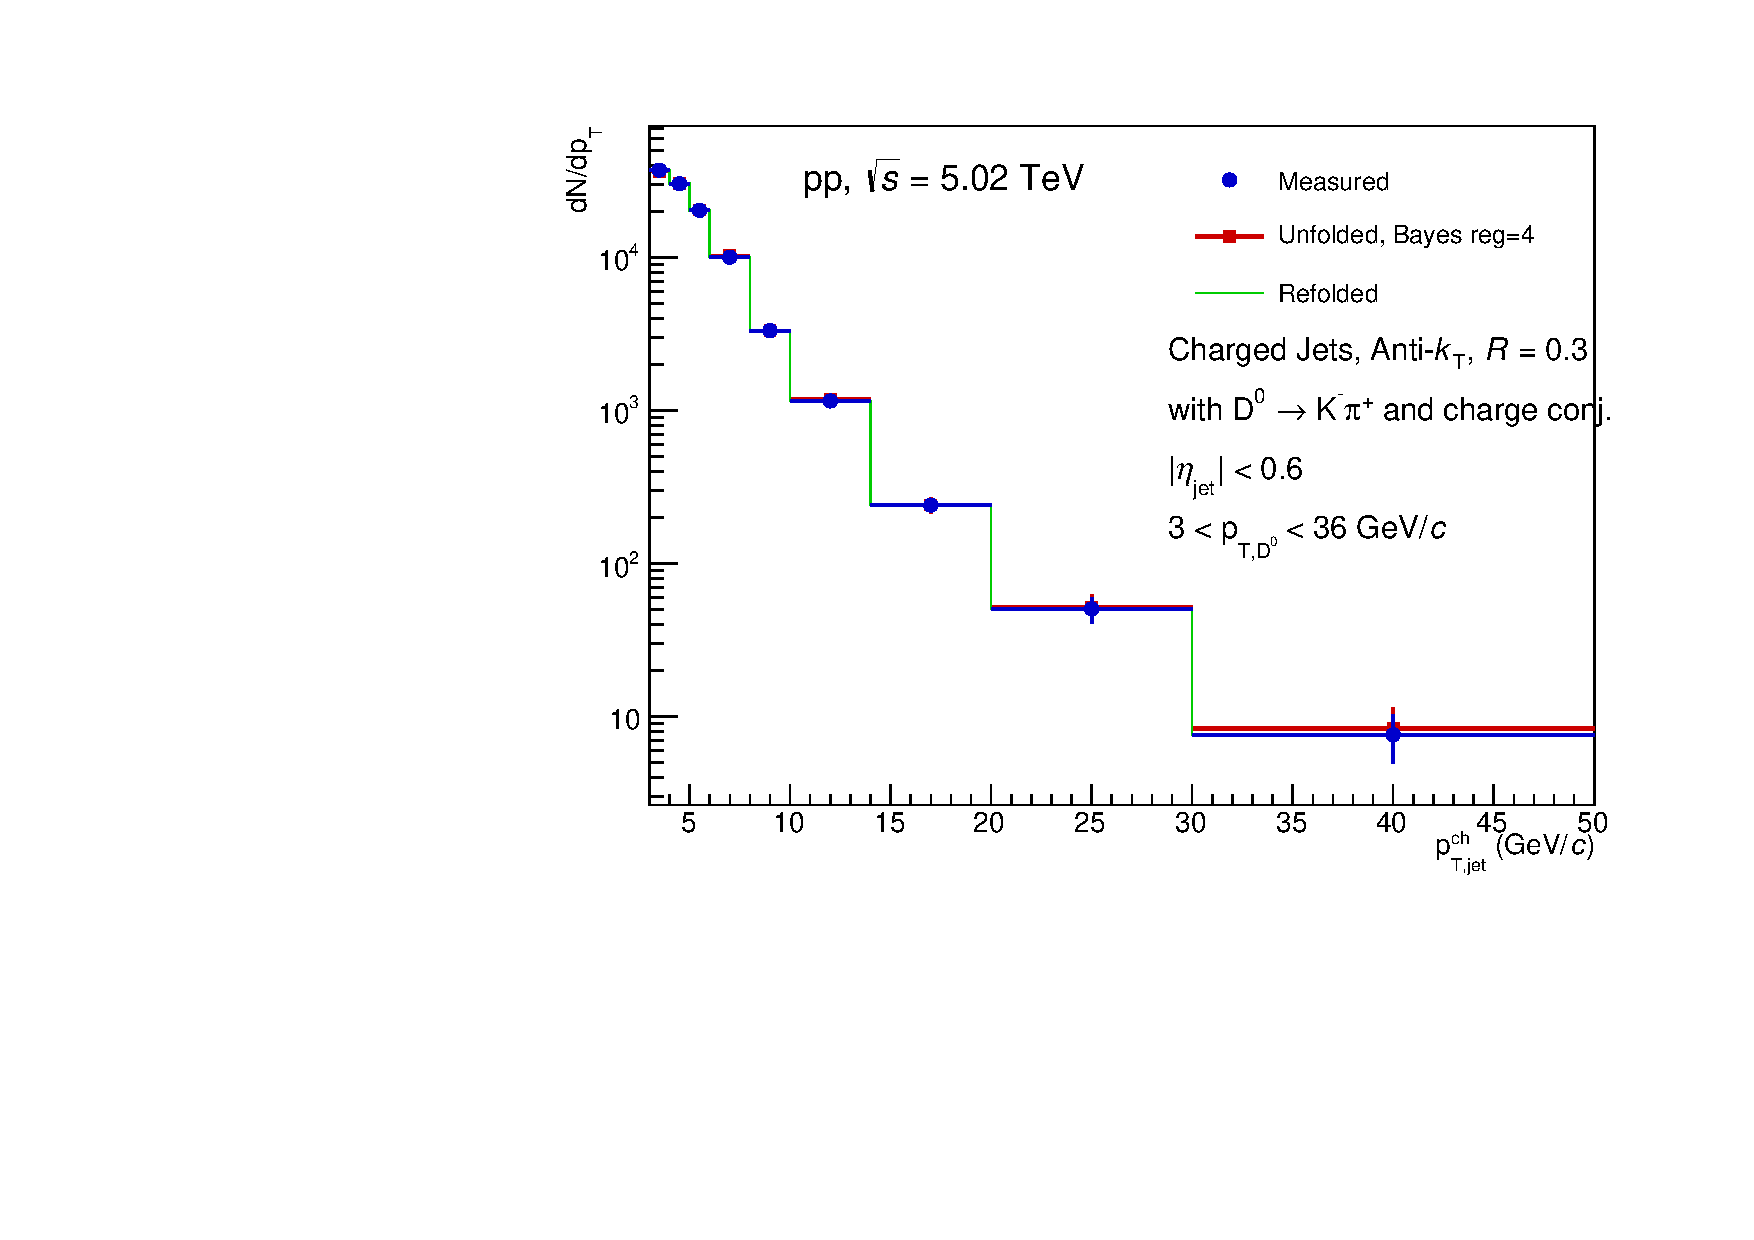
\includegraphics[width=0.53\textwidth]{/home/jackbauer/Work/alice/analysis/pp5TeV/D0jet/results_APW/Final_DzeroR02_paperCuts/Default/unfolding_Bayes_5/plots/unfoldedSpectrum_UnfSpectrum.pdf}
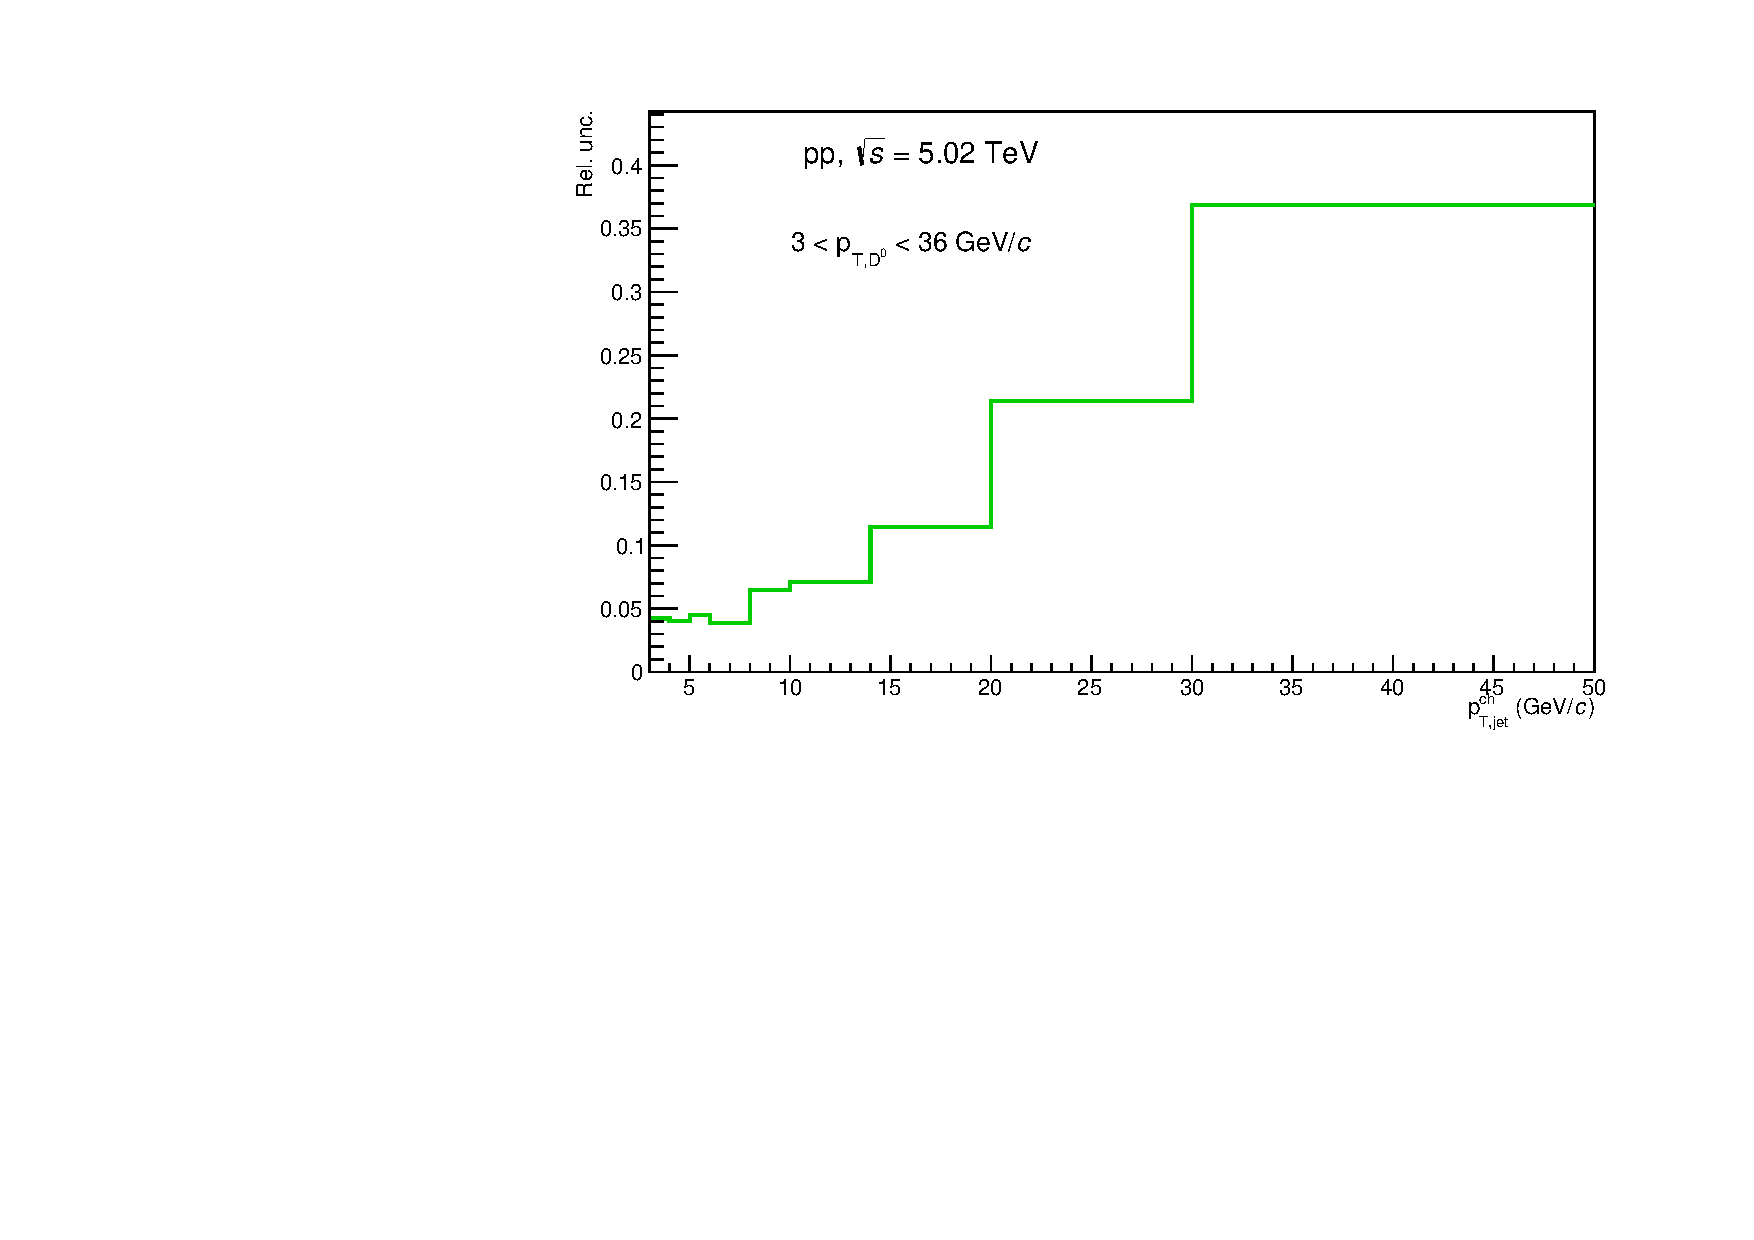
\includegraphics[width=0.46\textwidth]{/home/jackbauer/Work/alice/analysis/pp5TeV/D0jet/results_APW/Final_DzeroR02_paperCuts/Default/unfolding_Bayes_5/plots/unfoldedSpectrum_UnfSpectrum_unc.pdf}
\caption{R=0.2: Left: Corrected jet \pt spectrum before (blue) and after (red) the unfolding procedure (Bayesian method with 5 iterations). Right: Relative statistical uncertainties on the \Dzero-tagged jet \pt\ spectrum after unfolding.}
\label{fig:UnfSpec_pp_DzeroR02}
\end{figure}
\begin{figure}[bth]
\centering
\includegraphics[width=0.53\textwidth]{/home/jackbauer/Work/alice/analysis/pp5TeV/D0jet/results_APW/Final_DzeroR03_paperCuts/Default/unfolding_Bayes_5/plots/unfoldedSpectrum_UnfSpectrum.pdf}
\includegraphics[width=0.46\textwidth]{/home/jackbauer/Work/alice/analysis/pp5TeV/D0jet/results_APW/Final_DzeroR03_paperCuts/Default/unfolding_Bayes_5/plots/unfoldedSpectrum_UnfSpectrum_unc.pdf}
\caption{R=0.3: Left: Corrected jet \pt spectrum before (blue) and after (red) the unfolding procedure (Bayesian method with 5 iterations). Right: Relative statistical uncertainties on the \Dzero-tagged jet \pt\ spectrum after unfolding.}
\label{fig:UnfSpec_pp_DzeroR03}
\end{figure}
\begin{figure}[bth]
\centering
\includegraphics[width=0.53\textwidth]{/home/jackbauer/Work/alice/analysis/pp5TeV/D0jet/results_APW/Final_DzeroR04_paperCuts/Default/unfolding_Bayes_5/plots/unfoldedSpectrum_UnfSpectrum.pdf}
\includegraphics[width=0.46\textwidth]{/home/jackbauer/Work/alice/analysis/pp5TeV/D0jet/results_APW/Final_DzeroR04_paperCuts/Default/unfolding_Bayes_5/plots/unfoldedSpectrum_UnfSpectrum_unc.pdf}
\caption{R=0.4: Left: Corrected jet \pt spectrum before (blue) and after (red) the unfolding procedure (Bayesian method with 5 iterations). Right: Relative statistical uncertainties on the \Dzero-tagged jet \pt\ spectrum after unfolding.}
\label{fig:UnfSpec_pp_DzeroR04}
\end{figure}
\begin{figure}[bth]
\centering
\includegraphics[width=0.53\textwidth]{/home/jackbauer/Work/alice/analysis/pp5TeV/D0jet/results_APW/Final_DzeroR06_paperCuts/Default/unfolding_Bayes_5/plots/unfoldedSpectrum_UnfSpectrum.pdf}
\includegraphics[width=0.46\textwidth]{/home/jackbauer/Work/alice/analysis/pp5TeV/D0jet/results_APW/Final_DzeroR06_paperCuts/Default/unfolding_Bayes_5/plots/unfoldedSpectrum_UnfSpectrum_unc.pdf}
\caption{R=0.6: Left: Corrected jet \pt spectrum before (blue) and after (red) the unfolding procedure (Bayesian method with 5 iterations). Right: Relative statistical uncertainties on the \Dzero-tagged jet \pt\ spectrum after unfolding.}
\label{fig:UnfSpec_pp_DzeroR06}
\end{figure}
%%Folding comparisons

The green line represents refolded back spectrum. And different versions of the refolded spectrum resulting from considering different iterations for unfolding are compared to the measured jet-\pt\ spectrum before it could be unfolded in the right panel of Fig.~\ref{fig:unfIterations_pp_DzeroR02} for jet radius R=0.2. Figure~\ref{fig:unfIterations_pp_DzeroR02} (left) shows also unfolded spectra with next iterations compared to the default spectrum obtained with 5 iterations. Similar plots for other jet radii R=0.3, R=0.4 and R=0.6 are shown in figures~\ref{fig:unfIterations_pp_DzeroR03}, \ref{fig:unfIterations_pp_DzeroR04} and \ref{fig:unfIterations_pp_DzeroR06} respectively. The final reported jet \pt\ range is 5 $< \ptchjet<$ 50 \GeVc.
Comparison of unfolded spectra with the SVD method, different \pt\ ranges for the input and unfolded spectra, and different priors are presented in the systematic uncertainties section, see~\ref{sUnfoldSys}. 

\begin{figure}[bth]
\centering
\includegraphics[width=0.45\textwidth]{/home/jackbauer/Work/alice/analysis/pp5TeV/D0jet/results_APW/Final_DzeroR02_paperCuts/Default/unfolding_Bayes_5/plots/unfoldedSpectrum_unfRatio.pdf}
\includegraphics[width=0.45\textwidth]{/home/jackbauer/Work/alice/analysis/pp5TeV/D0jet/results_APW/Final_DzeroR02_paperCuts/Default/unfolding_Bayes_5/plots/unfoldedSpectrum_foldedRatio.pdf}
\caption{R=0.2: Left: ratio of the unfolded spectra for up to 10 iterations to the default unfolded spectrum with 5 iterations in the Bayesian unfolding. Right: ratio of the refolded spectrum for up to 10 iterations to the measured in the Bayesian unfolding. 
%The considered jet \pt\ range is above 5 \GeVc.
}
\label{fig:unfIterations_pp_DzeroR02}
\end{figure}

\begin{figure}[bth]
\centering
\includegraphics[width=0.45\textwidth]{/home/jackbauer/Work/alice/analysis/pp5TeV/D0jet/results_APW/Final_DzeroR03_paperCuts/Default/unfolding_Bayes_5/plots/unfoldedSpectrum_unfRatio.pdf}
\includegraphics[width=0.45\textwidth]{/home/jackbauer/Work/alice/analysis/pp5TeV/D0jet/results_APW/Final_DzeroR03_paperCuts/Default/unfolding_Bayes_5/plots/unfoldedSpectrum_foldedRatio.pdf}
\caption{R=0.3: Left: ratio of the unfolded spectra for up to 10 iterations to the default unfolded spectrum with 5 iterations in the Bayesian unfolding. Right: ratio of the refolded spectrum for up to 10 iterations to the measured in the Bayesian unfolding. 
%The considered jet \pt\ range is above 5 \GeVc.
}
\label{fig:unfIterations_pp_DzeroR03}
\end{figure}

\begin{figure}[bth]
\centering
\includegraphics[width=0.45\textwidth]{/home/jackbauer/Work/alice/analysis/pp5TeV/D0jet/results_APW/Final_DzeroR04_paperCuts/Default/unfolding_Bayes_5/plots/unfoldedSpectrum_unfRatio.pdf}
\includegraphics[width=0.45\textwidth]{/home/jackbauer/Work/alice/analysis/pp5TeV/D0jet/results_APW/Final_DzeroR04_paperCuts/Default/unfolding_Bayes_5/plots/unfoldedSpectrum_foldedRatio.pdf}
\caption{R=0.4: Left: ratio of the unfolded spectra for up to 10 iterations to the default unfolded spectrum with 5 iterations in the Bayesian unfolding. Right: ratio of the refolded spectrum for up to 10 iterations to the measured in the Bayesian unfolding. 
%The considered jet \pt\ range is above 5 \GeVc.
}
\label{fig:unfIterations_pp_DzeroR04}
\end{figure}

\begin{figure}[bth]
\centering
\includegraphics[width=0.45\textwidth]{/home/jackbauer/Work/alice/analysis/pp5TeV/D0jet/results_APW/Final_DzeroR06_paperCuts/Default/unfolding_Bayes_5/plots/unfoldedSpectrum_unfRatio.pdf}
\includegraphics[width=0.45\textwidth]{/home/jackbauer/Work/alice/analysis/pp5TeV/D0jet/results_APW/Final_DzeroR06_paperCuts/Default/unfolding_Bayes_5/plots/unfoldedSpectrum_foldedRatio.pdf}
\caption{R=0.6: Left: ratio of the unfolded spectra for up to 10 iterations to the default unfolded spectrum with 5 iterations in the Bayesian unfolding. Right: ratio of the refolded spectrum for up to 10 iterations to the measured in the Bayesian unfolding. 
%The considered jet \pt\ range is above 5 \GeVc.
}
\label{fig:unfIterations_pp_DzeroR06}
\end{figure}
%%%%%%%%%%%%%%%%%%%%
\section{Unfolding for jet \pt\ spectra: MC Closure test}
\label{sect:unfResults_jetClosure}
The analysis procedure needed to be validated using Monte Carlo simulations. This was done through a Monte Carlo closure test where the Monte Carlo sample was divided into two parts randomly: one was used to make the detector response matrix and the second was used to produce the detector level jet-\pt\ distribution and the true level jet-\pt\ distribution. The idea is to unfold the detector level distribution and compare the same with the true level distribution and therefore check how much was the closure. Both the distributions are unmatched; i.e. the full kinematic range of true level distribution was taken without any selection done to its detector level kinematic range. The detector level distribution was then scaled by reconstruction efficiencies as discussed in sec:\ref{sect:DmesonRecEff}. This test is especially done for the unfolding procedure because the Monte Carlo sample used is devoid of contribution from non-prompt D-jets and only contains the prompt fraction as we understand at the analysis step of unfolding in sec:\ref{sect:unfResults_jet}. The division of the full Monte Carlo sample into two was done so to avoid any correlation between the detector response matrix and efficiency scaled detector level distribution. Ten random trials were done. A ratio was taken between true level and unfolded detector level distributions for each trial. A root mean square of the ratios were taken as the final values for the closure test.

Figure \ref{fig:unfClosureJet_pp_DzeroR02} shows, for R=0.2, the ratios of each trial on the left and an RMS of the ratios on the right.
The corresponding plots for R=0.3, 0.4 and 0.6 are shown in figures \ref{fig:unfClosureJet_pp_DzeroR03}, \ref{fig:unfClosureJet_pp_DzeroR04} and \ref{fig:unfClosureJet_pp_DzeroR06} respectively.
\begin{figure}[bth]
\centering
\includegraphics[width=0.45\textwidth]{/home/jackbauer/ALICE_HeavyFlavour/work/Djets/alice_Djets/Djets/pySystematics_paper/jetxsec/plots/JET/9_Closure/9_Close02.pdf}
\includegraphics[width=0.45\textwidth]{/home/jackbauer/ALICE_HeavyFlavour/work/Djets/alice_Djets/Djets/pySystematics_paper/jetxsec/plots/JET/9_Closure/9_CloRMS02.pdf}
\caption{R=0.2: Left: ratio of the unfolded spectra to the true distribution with 5 iterations in the Bayesian unfolding. Right: RMS of the ratios from the left. 
}
\label{fig:unfClosureJet_pp_DzeroR02}
\end{figure}
\begin{figure}[bth]
\centering
\includegraphics[width=0.45\textwidth]{/home/jackbauer/ALICE_HeavyFlavour/work/Djets/alice_Djets/Djets/pySystematics_paper/jetxsec/plots/JET/9_Closure/9_Close03.pdf}
\includegraphics[width=0.45\textwidth]{/home/jackbauer/ALICE_HeavyFlavour/work/Djets/alice_Djets/Djets/pySystematics_paper/jetxsec/plots/JET/9_Closure/9_CloRMS03.pdf}
\caption{R=0.3: Left: ratio of the unfolded spectra to the true distribution with 5 iterations in the Bayesian unfolding. Right: RMS of the ratios from the left. 
}
\label{fig:unfClosureJet_pp_DzeroR03}
\end{figure}
\begin{figure}[bth]
\centering
\includegraphics[width=0.45\textwidth]{/home/jackbauer/ALICE_HeavyFlavour/work/Djets/alice_Djets/Djets/pySystematics_paper/jetxsec/plots/JET/9_Closure/9_Close04.pdf}
\includegraphics[width=0.45\textwidth]{/home/jackbauer/ALICE_HeavyFlavour/work/Djets/alice_Djets/Djets/pySystematics_paper/jetxsec/plots/JET/9_Closure/9_CloRMS04.pdf}
\caption{R=0.4: Left: ratio of the unfolded spectra to the true distribution with 5 iterations in the Bayesian unfolding. Right: RMS of the ratios from the left. 
}
\label{fig:unfClosureJet_pp_DzeroR04}
\end{figure}
\begin{figure}[bth]
\centering
\includegraphics[width=0.45\textwidth]{/home/jackbauer/ALICE_HeavyFlavour/work/Djets/alice_Djets/Djets/pySystematics_paper/jetxsec/plots/JET/9_Closure/9_Close06.pdf}
\includegraphics[width=0.45\textwidth]{/home/jackbauer/ALICE_HeavyFlavour/work/Djets/alice_Djets/Djets/pySystematics_paper/jetxsec/plots/JET/9_Closure/9_CloRMS06.pdf}
\caption{R=0.6: Left: ratio of the unfolded spectra to the true distribution with 5 iterations in the Bayesian unfolding. Right: RMS of the ratios from the left. 
}
\label{fig:unfClosureJet_pp_DzeroR06}
\end{figure}
%%%%%%%%%%%%%%%%%%%%%%%%%%%%%%%%%%%%%%%%%%%%%%%%%%%%%%%%%%%%%%%%%%%%%%
%%%%%%%%%%%%%%%%%%%%%%%%%%%%%%%%%%%%%%%%%%%%%%%%%%%%%%%%%%%%%%%%%%%%%%
\section{Systematic Uncertainties for jet-\pt\ spectra}

We considered the following sources of systematic uncertainties:

\begin{easylist}[itemize]
& Raw yield extraction
& D-Meson Selection Cuts
& B Feed-Down
& Unfolding
& Tracking Efficiency
& \pt\ Shape of the Monte Carlo Spectrum
\end{easylist}

\subsection{Raw Yield Extraction: Fitting procedure}
The stability and systematics of the raw yield extraction has been assessed on the lines of the \texttt{MultiTrial} framework developed by the D2H group. A fit of the invariant mass distribution is performed many times varying several conditions, such us binning, fixed vs. free parameters, background function, fit range. The following variations were included in the assessment of the systematics for the raw yield extraction of \Dzero jets in \pp:
\begin{itemize}
\item free $\sigma$(default), fixed $\sigma=\sigma_{\rm MC}$, fixed $\sigma=1.1\sigma_{\rm MC}$, fixed $\sigma=0.9\sigma_{\rm MC}$
\item background functions: exponential (default), linear, second-order polynomial;
\item free mass (default) and fixed $m_{0}=m_{\rm PDG}$;
\item lower limit of fit range: $1.71$, $1.72$ (default), $1.74$~\GeVcsq;
\item upper limit of fit range: $2.10$, $2.09$ (default), $2.11$~\GeVcsq;
\item rebin by factor 2, 4, 1(default)
\end{itemize}
So the total number of different multiple trials performed are 4 ($\sigma$ variations) $\times$ 3 (background variations) $\times$ 2 (mass variations) $\times$ 3 (lower limit of fit range variations) $\times$ 3 (upper limit of fit variations) $\times$ 3 (rebinning factors) = 648.

Starting with R=0.2, we see in figure \ref{fig:MTYieldsPerDptBin_pp_DzeroR02}, the raw jet-\pt\ distributions in each bin of D-\pt\ for all the trials. The yield against each trial per jet-\pt\ bin is shown in figure \ref{fig:MTYieldsPerJetBin_pp_DzeroR02}, and the frequency of the yields are shown in figure \ref{fig:MTYieldDistPerJetBin_pp_DzeroR02}. The jet-\pt\ distributions of summed yields are shown as a ratio to the default distribution on the left of figure \ref{fig:MTRatioRMS_pp_DzeroR02} and the right, their root-mean-square values are shown. The root-mean-square values represent the systematic uncertainties from multi-trial procedure of the raw yield extraction.

Corresponding plots for R=0.3 are in figures \ref{fig:MTYieldsPerDptBin_pp_DzeroR03}, \ref{fig:MTYieldsPerJetBin_pp_DzeroR03}, \ref{fig:MTYieldDistPerJetBin_pp_DzeroR03}, and \ref{fig:MTRatioRMS_pp_DzeroR03}.
For R=0.4, we have figures \ref{fig:MTYieldsPerDptBin_pp_DzeroR04}, \ref{fig:MTYieldsPerJetBin_pp_DzeroR04}, \ref{fig:MTYieldDistPerJetBin_pp_DzeroR04}, and \ref{fig:MTRatioRMS_pp_DzeroR04}.
And for R=0.6, we have figures \ref{fig:MTYieldsPerDptBin_pp_DzeroR06}, \ref{fig:MTYieldsPerJetBin_pp_DzeroR06}, \ref{fig:MTYieldDistPerJetBin_pp_DzeroR06}, and \ref{fig:MTRatioRMS_pp_DzeroR06}.
\begin{figure}[bth]
\centering
\includegraphics[width=\textwidth]{/home/jackbauer/ALICE_HeavyFlavour/work/Djets/alice_Djets/Djets/pySystematics_paper/jetxsec/plots/JET/0_Multi/0_Multi_02_sysRaw.pdf}
\caption{R=0.2}
\label{fig:MTYieldsPerDptBin_pp_DzeroR02}
\end{figure}
%%
\begin{figure}[bth]
\centering
\includegraphics[width=\textwidth]{/home/jackbauer/ALICE_HeavyFlavour/work/Djets/alice_Djets/Djets/pySystematics_paper/jetxsec/plots/JET/0_Multi/0_Multi_02_YieldTrials.pdf}
\caption{R=0.2
}
\label{fig:MTYieldsPerJetBin_pp_DzeroR02}
\end{figure}
%%
\begin{figure}[bth]
\centering
\includegraphics[width=\textwidth]{/home/jackbauer/ALICE_HeavyFlavour/work/Djets/alice_Djets/Djets/pySystematics_paper/jetxsec/plots/JET/0_Multi/0_Multi_02_yieldDist.pdf}
\caption{R=0.2
}
\label{fig:MTYieldDistPerJetBin_pp_DzeroR02}
\end{figure}
%%
\begin{figure}[bth]
\centering
\includegraphics[width=0.49\textwidth]{/home/jackbauer/ALICE_HeavyFlavour/work/Djets/alice_Djets/Djets/pySystematics_paper/jetxsec/plots/JET/0_Multi/0_Multi_02_sysRatio.pdf}
\includegraphics[width=0.49\textwidth]{/home/jackbauer/ALICE_HeavyFlavour/work/Djets/alice_Djets/Djets/pySystematics_paper/jetxsec/plots/JET/0_Multi/0_Multi_02_sysRMS.pdf}
\caption{R=0.2: Left: ratio of the multi-trial distributions to the default by Side-Band method. Right: RMS of the ratios from the left. 
}
\label{fig:MTRatioRMS_pp_DzeroR02}
\end{figure}

%%%%%%%%%%%%%   R=0.3
\begin{figure}[bth]
\centering
\includegraphics[width=\textwidth]{/home/jackbauer/ALICE_HeavyFlavour/work/Djets/alice_Djets/Djets/pySystematics_paper/jetxsec/plots/JET/0_Multi/0_Multi_03_sysRaw.pdf}
\caption{R=0.3}
\label{fig:MTYieldsPerDptBin_pp_DzeroR03}
\end{figure}
%%
\begin{figure}[bth]
\centering
\includegraphics[width=\textwidth]{/home/jackbauer/ALICE_HeavyFlavour/work/Djets/alice_Djets/Djets/pySystematics_paper/jetxsec/plots/JET/0_Multi/0_Multi_03_YieldTrials.pdf}
\caption{R=0.3
}
\label{fig:MTYieldsPerJetBin_pp_DzeroR03}
\end{figure}
%%
\begin{figure}[bth]
\centering
\includegraphics[width=\textwidth]{/home/jackbauer/ALICE_HeavyFlavour/work/Djets/alice_Djets/Djets/pySystematics_paper/jetxsec/plots/JET/0_Multi/0_Multi_03_yieldDist.pdf}
\caption{R=0.3}
\label{fig:MTYieldDistPerJetBin_pp_DzeroR03}
\end{figure}
%%
\begin{figure}[bth]
\centering
\includegraphics[width=0.49\textwidth]{/home/jackbauer/ALICE_HeavyFlavour/work/Djets/alice_Djets/Djets/pySystematics_paper/jetxsec/plots/JET/0_Multi/0_Multi_03_sysRatio.pdf}
\includegraphics[width=0.49\textwidth]{/home/jackbauer/ALICE_HeavyFlavour/work/Djets/alice_Djets/Djets/pySystematics_paper/jetxsec/plots/JET/0_Multi/0_Multi_03_sysRMS.pdf}
\caption{R=0.3: Left: ratio of the multi-trial distributions to the default by Side-Band method. Right: RMS of the ratios from the left. 
}
\label{fig:MTRatioRMS_pp_DzeroR03}
\end{figure}

%%%%%%%%%%%%%   R=0.4
\begin{figure}[bth]
\centering
\includegraphics[width=\textwidth]{/home/jackbauer/ALICE_HeavyFlavour/work/Djets/alice_Djets/Djets/pySystematics_paper/jetxsec/plots/JET/0_Multi/0_Multi_04_sysRaw.pdf}
\caption{R=0.4}
\label{fig:MTYieldsPerDptBin_pp_DzeroR04}
\end{figure}
%%
\begin{figure}[bth]
\centering
\includegraphics[width=\textwidth]{/home/jackbauer/ALICE_HeavyFlavour/work/Djets/alice_Djets/Djets/pySystematics_paper/jetxsec/plots/JET/0_Multi/0_Multi_04_YieldTrials.pdf}
\caption{R=0.4
}
\label{fig:MTYieldsPerJetBin_pp_DzeroR04}
\end{figure}
%%
\begin{figure}[bth]
\centering
\includegraphics[width=\textwidth]{/home/jackbauer/ALICE_HeavyFlavour/work/Djets/alice_Djets/Djets/pySystematics_paper/jetxsec/plots/JET/0_Multi/0_Multi_04_yieldDist.pdf}
\caption{R=0.4}
\label{fig:MTYieldDistPerJetBin_pp_DzeroR04}
\end{figure}
%%
\begin{figure}[bth]
\centering
\includegraphics[width=0.49\textwidth]{/home/jackbauer/ALICE_HeavyFlavour/work/Djets/alice_Djets/Djets/pySystematics_paper/jetxsec/plots/JET/0_Multi/0_Multi_04_sysRatio.pdf}
\includegraphics[width=0.49\textwidth]{/home/jackbauer/ALICE_HeavyFlavour/work/Djets/alice_Djets/Djets/pySystematics_paper/jetxsec/plots/JET/0_Multi/0_Multi_04_sysRMS.pdf}
\caption{R=0.4: Left: ratio of the multi-trial distributions to the default by Side-Band method. Right: RMS of the ratios from the left. 
}
\label{fig:MTRatioRMS_pp_DzeroR04}
\end{figure}

%%%%%%%%%%%%%   R=0.6
\begin{figure}[bth]
\centering
\includegraphics[width=\textwidth]{/home/jackbauer/ALICE_HeavyFlavour/work/Djets/alice_Djets/Djets/pySystematics_paper/jetxsec/plots/JET/0_Multi/0_Multi_06_sysRaw.pdf}
\caption{R=0.6}
\label{fig:MTYieldsPerDptBin_pp_DzeroR06}
\end{figure}
%%
\begin{figure}[bth]
\centering
\includegraphics[width=\textwidth]{/home/jackbauer/ALICE_HeavyFlavour/work/Djets/alice_Djets/Djets/pySystematics_paper/jetxsec/plots/JET/0_Multi/0_Multi_06_YieldTrials.pdf}
\caption{R=0.6
}
\label{fig:MTYieldsPerJetBin_pp_DzeroR06}
\end{figure}
%%
\begin{figure}[bth]
\centering
\includegraphics[width=\textwidth]{/home/jackbauer/ALICE_HeavyFlavour/work/Djets/alice_Djets/Djets/pySystematics_paper/jetxsec/plots/JET/0_Multi/0_Multi_06_yieldDist.pdf}
\caption{R=0.6}
\label{fig:MTYieldDistPerJetBin_pp_DzeroR06}
\end{figure}
%%
\begin{figure}[bth]
\centering
\includegraphics[width=0.49\textwidth]{/home/jackbauer/ALICE_HeavyFlavour/work/Djets/alice_Djets/Djets/pySystematics_paper/jetxsec/plots/JET/0_Multi/0_Multi_06_sysRatio.pdf}
\includegraphics[width=0.49\textwidth]{/home/jackbauer/ALICE_HeavyFlavour/work/Djets/alice_Djets/Djets/pySystematics_paper/jetxsec/plots/JET/0_Multi/0_Multi_06_sysRMS.pdf}
\caption{R=0.6: Left: ratio of the multi-trial distributions to the default by Side-Band method. Right: RMS of the ratios from the left. 
}
\label{fig:MTRatioRMS_pp_DzeroR06}
\end{figure}
\FloatBarrier
%%%%%%%%%%%%%%%%%%%%%%%%%%%%%%%%%%%%%%%%%%%%%%%%%%%%%%%%%%
\subsection{Raw Yield Extraction: Variation of signal and side-band ranges}
As an additional systematic uncertainty, variations of ranges of the signal and side-band definitions in the invariant-mass fit procedure are considered. The signal windows considered are 2$\sigma$ and 3$\sigma$, while the side-band background windows are considered with the larger extent being 8$\sigma$, 9$\sigma$ and the lower extent being 3.5$\sigma$, 4$\sigma$ and 4.5$\sigma$.
Figure~\ref{fig:JetPtSys_Dzero_SBvariatonR02} shows ratios of efficiency corrected yields to the central value and RMS of the variations as systematic uncertainties for R=0.2. For R=0.3, 0.4 and 0.6, the plots are in figures~\ref{fig:JetPtSys_Dzero_SBvariatonR03}, \ref{fig:JetPtSys_Dzero_SBvariatonR04}, and \ref{fig:JetPtSys_Dzero_SBvariatonR06} respectively.
\begin{figure}[bth]
\begin{center}
\includegraphics[width=0.49\textwidth]{/home/jackbauer/ALICE_HeavyFlavour/work/Djets/alice_Djets/Djets/pySystematics_paper/jetxsec/plots/JET/2_SigSB/2_SigSB_sys02.pdf}
\includegraphics[width=0.49\textwidth]{/home/jackbauer/ALICE_HeavyFlavour/work/Djets/alice_Djets/Djets/pySystematics_paper/jetxsec/plots/JET/2_SigSB/2_SigSB_sysRMS02.pdf}
\caption{Left: ratio of different distributions due to variation in signal and side-band ranges. Right: RMS of the ratios from left as systematic uncertainties.} 
\label{fig:JetPtSys_Dzero_SBvariatonR02}
\end{center}
\end{figure}
%%%
\begin{figure}[bth]
\begin{center}
\includegraphics[width=0.49\textwidth]{/home/jackbauer/ALICE_HeavyFlavour/work/Djets/alice_Djets/Djets/pySystematics_paper/jetxsec/plots/JET/2_SigSB/2_SigSB_sys03.pdf}
\includegraphics[width=0.49\textwidth]{/home/jackbauer/ALICE_HeavyFlavour/work/Djets/alice_Djets/Djets/pySystematics_paper/jetxsec/plots/JET/2_SigSB/2_SigSB_sysRMS03.pdf}
\caption{Left: ratio of different distributions due to variation in signal and side-band ranges. Right: RMS of the ratios from left as systematic uncertainties.} 
\label{fig:JetPtSys_Dzero_SBvariatonR03}
\end{center}
\end{figure}
%%%
\begin{figure}[bth]
\begin{center}
\includegraphics[width=0.49\textwidth]{/home/jackbauer/ALICE_HeavyFlavour/work/Djets/alice_Djets/Djets/pySystematics_paper/jetxsec/plots/JET/2_SigSB/2_SigSB_sys04.pdf}
\includegraphics[width=0.49\textwidth]{/home/jackbauer/ALICE_HeavyFlavour/work/Djets/alice_Djets/Djets/pySystematics_paper/jetxsec/plots/JET/2_SigSB/2_SigSB_sysRMS04.pdf}
\caption{Left: ratio of different distributions due to variation in signal and side-band ranges. Right: RMS of the ratios from left as systematic uncertainties.} 
\label{fig:JetPtSys_Dzero_SBvariatonR04}
\end{center}
\end{figure}
%%%
\begin{figure}[bth]
\begin{center}
\includegraphics[width=0.49\textwidth]{/home/jackbauer/ALICE_HeavyFlavour/work/Djets/alice_Djets/Djets/pySystematics_paper/jetxsec/plots/JET/2_SigSB/2_SigSB_sys06.pdf}
\includegraphics[width=0.49\textwidth]{/home/jackbauer/ALICE_HeavyFlavour/work/Djets/alice_Djets/Djets/pySystematics_paper/jetxsec/plots/JET/2_SigSB/2_SigSB_sysRMS06.pdf}
\caption{Left: ratio of different distributions due to variation in signal and side-band ranges. Right: RMS of the ratios from left as systematic uncertainties.} 
\label{fig:JetPtSys_Dzero_SBvariatonR06}
\end{center}
\end{figure}
%%%%%%%%%% reflection
\FloatBarrier
\subsection{Raw Yield Extraction: Variation of reflection to signal ratio}\label{subsec:reflection}

By default, the ratio reflection/signal is a fixed parameter in the fit and is taken from the MC simulation. The reflection/signal ratio is varied to estimate the systematic uncertainty. Considered variations are $\pm$ 50\% of the default value. Systematic uncertainties, which are the maximum from each bin, arising from these variation on the final unfolded jet \pt\ spectra are  about 1-3\%, as shown in Fig.~\ref{fig:JetPtSys_Dzero_ReflR02R03} and ~\ref{fig:JetPtSys_Dzero_ReflR04R06}.
%The uncertainties are added in quadratures in order to obtain the final systematic uncertainty on the raw yield extraction. 
\begin{figure}[bth]
\begin{center}
\includegraphics[width=0.45\textwidth]{/home/jackbauer/ALICE_HeavyFlavour/work/Djets/alice_Djets/Djets/pySystematics_paper/jetxsec/plots/JET/1_Ref/1_Ref_rat02.pdf}
\includegraphics[width=0.45\textwidth]{/home/jackbauer/ALICE_HeavyFlavour/work/Djets/alice_Djets/Djets/pySystematics_paper/jetxsec/plots/JET/1_Ref/1_Ref_rat03.pdf}
\caption{Left: R=0.2, right: R=0.3. Ratio of unfolded jet-\pt\ spectrum with $\pm$50\% variations of the reflection/signal ratio. Systematic uncertainties: maximum of the variations in each bin.} 
\label{fig:JetPtSys_Dzero_ReflR02R03}
\end{center}
\end{figure}
\begin{figure}[bth]
\begin{center}
\includegraphics[width=0.45\textwidth]{/home/jackbauer/ALICE_HeavyFlavour/work/Djets/alice_Djets/Djets/pySystematics_paper/jetxsec/plots/JET/1_Ref/1_Ref_rat04.pdf}
\includegraphics[width=0.45\textwidth]{/home/jackbauer/ALICE_HeavyFlavour/work/Djets/alice_Djets/Djets/pySystematics_paper/jetxsec/plots/JET/1_Ref/1_Ref_rat06.pdf}
\caption{Left: R=0.4, right: R=0.6. Ratio of unfolded jet-\pt\ spectrum with $\pm$50\% variations of the reflection/signal ratio. Systematic uncertainties: maximum of the variations in each bin.} 
\label{fig:JetPtSys_Dzero_ReflR04R06}
\end{center}
\end{figure}
%%%%%%%%%%%%%%%%%%%%%%%%%%%%%%%%%%%%%%%%%%%%%%%%%%%%%%%%%%%%
%%%%%%%%%%%%%% SELECTION CUTS
%%%%%%%%%%%%%%%%%%%%%%%%%%%%%%%%%%%%%%%%%%%%%%%%%%%%%%%%%%%%
\subsection{D-Meson Selection Cuts}
Uncertainties of the D-meson cut selection is estimated by varying cuts applied in the analysis of D-meson selection criteria, as reported in~\ref{sec:DmesonSel}. 

Four variations of cut selections of varying degrees of looseness or tightness to the default set of selection cuts are considered. The variations are chosen so that they vary \Dzero reconstruction efficiency to high enough extent so that a possible imperfection in MC simulation can be probed, though at high \ptd\ the selection criteria are already rather loose.
\Dzero-jet \pt\ distributions were obtained post B-feed down correction with these different cut sets. Their ratios to the default set are obtained and shown on the left panel while the RMS values for systematic uncertainties are shown on the right panel in each of the figures \ref{fig:JetPtCutSys_DzeroR02}, \ref{fig:JetPtCutSys_DzeroR03}, \ref{fig:JetPtCutSys_DzeroR04} and \ref{fig:JetPtCutSys_DzeroR06} for R=0.2, 0.3, 0.4 and 0.6 respectively. For R=0.2, the cuts -1 and -2 result in too much instability for the highest \pt\ bin. The results are obtained ignoring them for said jet-radius.

% and corresponding \Dzero-jet efficiencies are shown in Fig.~\ref{fig:JetPtRawSys_Dzero}, and ratios to the default set of cuts in Fig.~\ref{fig:JetPtRawSysRatio_Dzero}.
%Figure~\ref{fig:JetcutVarFD_Dzero} shows non-prompt \Dzero-jet reconstruction efficiencies for all the cut variations, and the variations of the FD fraction in the inclusive \Dzero-jet spectrum.

\begin{figure}[bth]
\begin{center}
\includegraphics[width=0.32\textwidth]{/home/jackbauer/ALICE_HeavyFlavour/work/Djets/alice_Djets/Djets/pySystematics_paper/jetxsec/plots/JET/3_Cuts/3_Cuts_ratio02.pdf}
\includegraphics[width=0.32\textwidth]{/home/jackbauer/ALICE_HeavyFlavour/work/Djets/alice_Djets/Djets/pySystematics_paper/jetxsec/plots/JET/3_Cuts/3_Cuts_sysRMS02.pdf}
\includegraphics[width=0.32\textwidth]{/home/jackbauer/ALICE_HeavyFlavour/work/Djets/alice_Djets/Djets/pySystematics_paper/jetxsec/plots/JET/3_Cuts/3_Cut_FIT02.pdf}
\caption{Left: ratios of \Dzero-jet \pt\ distributions with different cut sets to the default cut set. Right: corresponding root-mean-square of the ratios.} 
\label{fig:JetPtCutSys_DzeroR02}
\end{center}
\end{figure}

\begin{figure}[bth]
\begin{center}
\includegraphics[width=0.32\textwidth]{/home/jackbauer/ALICE_HeavyFlavour/work/Djets/alice_Djets/Djets/pySystematics_paper/jetxsec/plots/JET/3_Cuts/3_Cuts_ratio03.pdf}
\includegraphics[width=0.32\textwidth]{/home/jackbauer/ALICE_HeavyFlavour/work/Djets/alice_Djets/Djets/pySystematics_paper/jetxsec/plots/JET/3_Cuts/3_Cuts_sysRMS03.pdf}
\includegraphics[width=0.32\textwidth]{/home/jackbauer/ALICE_HeavyFlavour/work/Djets/alice_Djets/Djets/pySystematics_paper/jetxsec/plots/JET/3_Cuts/3_Cut_FIT03.pdf}
\caption{Left: ratios of \Dzero-jet \pt\ distributions with different cut sets to the default cut set. Right: corresponding root-mean-square of the ratios.} 
\label{fig:JetPtCutSys_DzeroR03}
\end{center}
\end{figure}


\begin{figure}[bth]
\begin{center}
\includegraphics[width=0.32\textwidth]{/home/jackbauer/ALICE_HeavyFlavour/work/Djets/alice_Djets/Djets/pySystematics_paper/jetxsec/plots/JET/3_Cuts/3_Cuts_ratio04.pdf}
\includegraphics[width=0.32\textwidth]{/home/jackbauer/ALICE_HeavyFlavour/work/Djets/alice_Djets/Djets/pySystematics_paper/jetxsec/plots/JET/3_Cuts/3_Cuts_sysRMS04.pdf}
\includegraphics[width=0.32\textwidth]{/home/jackbauer/ALICE_HeavyFlavour/work/Djets/alice_Djets/Djets/pySystematics_paper/jetxsec/plots/JET/3_Cuts/3_Cut_FIT04.pdf}
\caption{Left: ratios of \Dzero-jet \pt\ distributions with different cut sets to the default cut set. Right: corresponding root-mean-square of the ratios.} 
\label{fig:JetPtCutSys_DzeroR04}
\end{center}
\end{figure}

\begin{figure}[bth]
\begin{center}
\includegraphics[width=0.32\textwidth]{/home/jackbauer/ALICE_HeavyFlavour/work/Djets/alice_Djets/Djets/pySystematics_paper/jetxsec/plots/JET/3_Cuts/3_Cuts_ratio06.pdf}
\includegraphics[width=0.32\textwidth]{/home/jackbauer/ALICE_HeavyFlavour/work/Djets/alice_Djets/Djets/pySystematics_paper/jetxsec/plots/JET/3_Cuts/3_Cuts_sysRMS06.pdf}
\includegraphics[width=0.32\textwidth]{/home/jackbauer/ALICE_HeavyFlavour/work/Djets/alice_Djets/Djets/pySystematics_paper/jetxsec/plots/JET/3_Cuts/3_Cut_FIT06.pdf}
\caption{Left: ratios of \Dzero-jet \pt\ distributions with different cut sets to the default cut set. Right: corresponding root-mean-square of the ratios.} 
\label{fig:JetPtCutSys_DzeroR06}
\end{center}
\end{figure}
%%%%%%%%%%%%%%%%%%%%%%%%%%%%%%%%%%%%%%%
%%%%%%%%%  B FEED DOWN
%%%%%%%%%%%%%%%%%%%%%%%%%%%%%%%%%%%%%%%
\subsection{B Feed-Down Correction}\label{subsec:bfeedsys}

The B Feed-Down (FD) cross section is obtained from simulation with POWHEG+PYTHIA6 with EventGen decayer, as discussed in Section~\ref{sec:FD}.
In order to assess the systematic uncertainty the same simulation is performed with different choices of the quark mass $m_{\rm b}$, the factorization scale factor $\mu_{\rm F}$, and the renormalization scale factor $\mu_{\rm R}$.
Table~\ref{tab:FDpars} shows the list of parameters used to determine the central points and the variations used to determine the systematic uncertainty.
%As an additional variation the EvtGen is used as a decayer instead of Pytha6 {\color{red} THIS SHOULD BE ADDED TO THE SIMULATIONS}. 

\begin{table}[bth]
\caption{Parameters of the POWHEG+PYTHIA6+EventGen simulations for estimating B Feed-Down.}
     \label{tab:FDpars}
\begin{center}
    \begin{tabular}{lrr}
    \hline
    Parameter & Central Value & Variations \\ \hline
    $m_{\rm b}$ & $4.75$~\GeVcsq & $4.5$, $5.0$~\GeVcsq \\ 
    PDF & CT10nlo (21200) & -- \\ 
    ($\mu_{\rm F}$, $\mu_{\rm R}$) & (1,1) & (0.5,0.5), (0.5, 1), (1, 0.5), (2,2), (2,1), (1,2)
    \end{tabular}
    \end{center}
    \end{table}

The non-prompt \Dzero-jet \pt\ spectra after correcting for the efficiency and smearing with the detector effects are shown in on the left panels of Fig.~\ref{fig:ppFD_corr_DzeroR02}, ~\ref{fig:ppFD_corr_DzeroR03}, ~\ref{fig:ppFD_corr_DzeroR04} and ~\ref{fig:ppFD_corr_DzeroR06}, together with systematic uncertainties obtained by taking the largest upward and downward variation from the central point in each bin. Therefore, the shown uncertainties are asymmetric as seen in Fig.~\ref{fig:BFD_sysUnc_DzeroR02}, ~\ref{fig:BFD_sysUnc_DzeroR03}, ~\ref{fig:BFD_sysUnc_DzeroR04} and ~\ref{fig:BFD_sysUnc_DzeroR06}.

\begin{figure}
\centering
\begin{minipage}{.5\textwidth}
  \centering
  \includegraphics[width=\linewidth]{/home/jackbauer/ALICE_HeavyFlavour/work/Djets/alice_Djets/Djets/pySystematics_paper/jetxsec/plots/4_FD/4_FD_sys02.pdf}
  \caption{R=0.2: B feed-down sys. unc.}%{Systematic uncertainties after}\\ \centerline{B feed-down subtraction for R=0.2.}}
  \label{fig:BFD_sysUnc_DzeroR02}
\end{minipage}%
\begin{minipage}{.5\textwidth}
  \centering
  \includegraphics[width=\linewidth]{/home/jackbauer/ALICE_HeavyFlavour/work/Djets/alice_Djets/Djets/pySystematics_paper/jetxsec/plots/4_FD/4_FD_sys03.pdf}
  \caption{R=0.3: B feed-down sys. unc.}%{Systematic uncertainties after}\\ \centerline{B feed-down subtraction for R=0.3.}}
  \label{fig:BFD_sysUnc_DzeroR03}
\end{minipage}
\end{figure}
\begin{figure}
\centering
\begin{minipage}{.5\textwidth}
  \centering
  \includegraphics[width=\linewidth]{/home/jackbauer/ALICE_HeavyFlavour/work/Djets/alice_Djets/Djets/pySystematics_paper/jetxsec/plots/4_FD/4_FD_sys04.pdf}
  \caption{R=0.4: B feed-down sys. unc.}% after}\\ \centerline{B feed-down subtraction for R=0.4.}}
  \label{fig:BFD_sysUnc_DzeroR04}
\end{minipage}%
\begin{minipage}{.5\textwidth}
  \centering
  \includegraphics[width=\linewidth]{/home/jackbauer/ALICE_HeavyFlavour/work/Djets/alice_Djets/Djets/pySystematics_paper/jetxsec/plots/4_FD/4_FD_sys06.pdf}
  \caption{R=0.6: B feed-down sys. unc.}%{Systematic uncertainties after}\\ \centerline{B feed-down subtraction for R=0.6.}}
  \label{fig:BFD_sysUnc_DzeroR06}
\end{minipage}
\end{figure}
%%%%%%%%%%%%% unfolding Bayes priors
%%%%%%%%%%%%%%%%%%%%%%%
\clearpage
\subsection{Unfolding: Bayes unfolding with different priors}
\label{sUnfoldSysBayesPrior}
Unfolded \Dzero-jet \pt\ spectrum using the Bayesian method with 5 iterations was shown in Fig.~\ref{fig:UnfSpec_pp_DzeroR02}, ~\ref{fig:UnfSpec_pp_DzeroR03}, ~\ref{fig:UnfSpec_pp_DzeroR04} and ~\ref{fig:UnfSpec_pp_DzeroR06}. The baseline prior used for unfolding was the spectrum obtained at the generator level from PYTHIA. For the variations, the priors were obtained from a modified power-law function: 
\begin{equation}
f(\ptjet) = \ptjet^{-a}e^{-\frac{ab}{\ptjet}},
\end{equation}
where $a$ is the power-law index and $b$ is the position of the local maximum of the distribution. The exponential factor $e^{-\frac{ab}{\ptjet}}$ was added to avoid infinities at zero and have a more realistic spectrum (the physical cross-section goes to zero for $\ptjet \to 0$).
Used variations are: -prior0: $a=4.6$ $b=4$~\GeVc, prior1: $a=3$ $b=4$~\GeVc, prior2: $a=4$ $b=4$~\GeVc, prior3: $a=5$ $b=4$~\GeVc, prior4: $a=6$ $b=4$~\GeVc, prior5: $a=7$ $b=4$~\GeVc, prior6: $a=4.5$ $b=3$~\GeVc, prior7: $a=4.5$ $b=5$~\GeVc, prior8: fit to the measured spectrum. With new yields from unfolding with different priors, ratios were taken (see ~\ref{fig:sub1BayesPriorSysUncR02},  ~\ref{fig:sub1BayesPriorSysUncR03},  ~\ref{fig:sub1BayesPriorSysUncR04} and ~\ref{fig:sub1BayesPriorSysUncR06}) and their root-mean-square values (~\ref{fig:sub2BayesPriorSysUncR02}, ~\ref{fig:sub2BayesPriorSysUncR03}, ~\ref{fig:sub2BayesPriorSysUncR04} and ~\ref{fig:sub2BayesPriorSysUncR06}) were finalised as systematic uncertainties for all four jet-radii.

\begin{figure}
\centering
\begin{subfigure}{.5\textwidth}
  \centering
  \includegraphics[width=\linewidth]{/home/jackbauer/ALICE_HeavyFlavour/work/Djets/alice_Djets/Djets/pySystematics_paper/jetxsec/plots/JET/6_Priors/6_Priors_ratio02.pdf}
  \caption{Ratio of Bayes unfolded spectra from different priors to one from default prior.}
  \label{fig:sub1BayesPriorSysUncR02}
\end{subfigure}%
\begin{subfigure}{.5\textwidth}
  \centering
  \includegraphics[width=\linewidth]{/home/jackbauer/ALICE_HeavyFlavour/work/Djets/alice_Djets/Djets/pySystematics_paper/jetxsec/plots/JET/6_Priors/6_Priors_RMS02.pdf}
  \caption{Root-mean-square deviation for the ratios.}
  \label{fig:sub2BayesPriorSysUncR02}
\end{subfigure}
\caption{R=0.2: Systematic uncertainty from Bayes unfolding with different priors.}
  \label{fig:BayesPriorSysUncR02}
\end{figure}

\begin{figure}
\centering
\begin{subfigure}{.5\textwidth}
  \centering
  \includegraphics[width=\linewidth]{/home/jackbauer/ALICE_HeavyFlavour/work/Djets/alice_Djets/Djets/pySystematics_paper/jetxsec/plots/JET/6_Priors/6_Priors_ratio03.pdf}
  \caption{Ratio of Bayes unfolded spectra from different priors to one from default prior.}
  \label{fig:sub1BayesPriorSysUncR03}
\end{subfigure}%
\begin{subfigure}{.5\textwidth}
  \centering
  \includegraphics[width=\linewidth]{/home/jackbauer/ALICE_HeavyFlavour/work/Djets/alice_Djets/Djets/pySystematics_paper/jetxsec/plots/JET/6_Priors/6_Priors_RMS03.pdf}
  \caption{Root-mean-square deviation for the ratios.}
  \label{fig:sub2BayesPriorSysUncR03}
\end{subfigure}
\caption{R=0.3: Systematic uncertainty from Bayes unfolding with different priors.}
  \label{fig:BayesPriorSysUncR03}
\end{figure}

\begin{figure}
\centering
\begin{subfigure}{.5\textwidth}
  \centering
  \includegraphics[width=\linewidth]{/home/jackbauer/ALICE_HeavyFlavour/work/Djets/alice_Djets/Djets/pySystematics_paper/jetxsec/plots/JET/6_Priors/6_Priors_ratio04.pdf}
  \caption{Ratio of Bayes unfolded spectra from different priors to one from default prior.}
  \label{fig:sub1BayesPriorSysUncR04}
\end{subfigure}%
\begin{subfigure}{.5\textwidth}
  \centering
  \includegraphics[width=\linewidth]{/home/jackbauer/ALICE_HeavyFlavour/work/Djets/alice_Djets/Djets/pySystematics_paper/jetxsec/plots/JET/6_Priors/6_Priors_RMS04.pdf}
  \caption{Root-mean-square deviation for the ratios.}
  \label{fig:sub2BayesPriorSysUncR04}
\end{subfigure}
\caption{R=0.4: Systematic uncertainty from Bayes unfolding with different priors.}
  \label{fig:BayesPriorSysUncR04}
\end{figure}

\begin{figure}
\centering
\begin{subfigure}{.5\textwidth}
  \centering
  \includegraphics[width=\linewidth]{/home/jackbauer/ALICE_HeavyFlavour/work/Djets/alice_Djets/Djets/pySystematics_paper/jetxsec/plots/JET/6_Priors/6_Priors_ratio06.pdf}
  \caption{Ratio of Bayes unfolded spectra from different priors to one from default prior.}
  \label{fig:sub1BayesPriorSysUncR06}
\end{subfigure}%
\begin{subfigure}{.5\textwidth}
  \centering
  \includegraphics[width=\linewidth]{/home/jackbauer/ALICE_HeavyFlavour/work/Djets/alice_Djets/Djets/pySystematics_paper/jetxsec/plots/JET/6_Priors/6_Priors_RMS06.pdf}
  \caption{Root-mean-square deviation for the ratios.}
  \label{fig:sub2BayesPriorSysUncR06}
\end{subfigure}
\caption{R=0.6: Systematic uncertainty from Bayes unfolding with different priors.}
  \label{fig:BayesPriorSysUncR06}
\end{figure}
%%%%%%%%%%%%% unfolding Bayes iterations
%%%%%%%%%%%%%%%%%%%%%%%

\subsection{Unfolding: Bayes unfolding with different iterations}
\label{sUnfoldSysBayesIter}
In Bayesian unfolding, we used five iterations for the default method. As a source of systematic uncertainties, the number of iterations were changed by plus or minus one from the default value of five. This variation is shown in Fig.~\ref{fig:sub1BayesIterSysUncR02}, ~\ref{fig:sub1BayesIterSysUncR03}, ~\ref{fig:sub1BayesIterSysUncR04} and ~\ref{fig:sub1BayesIterSysUncR06}. Their root-mean-square values are taken as systematic uncertainties for corresponding jet radii as shown in Fig.~\ref{fig:sub2BayesIterSysUncR02}, ~\ref{fig:sub2BayesIterSysUncR03}, ~\ref{fig:sub2BayesIterSysUncR04} and ~\ref{fig:sub2BayesIterSysUncR06}.

\begin{figure}
\centering
\begin{subfigure}{.5\textwidth}
  \centering
  \includegraphics[width=\linewidth]{/home/jackbauer/ALICE_HeavyFlavour/work/Djets/alice_Djets/Djets/pySystematics_paper/jetxsec/plots/5_Iter/5_Iter_ratio02.pdf}
  \caption{Ratio of Bayes unfolded spectra from different iterations to one from default iteration.}
  \label{fig:sub1BayesIterSysUncR02}
\end{subfigure}%
\begin{subfigure}{.5\textwidth}
  \centering
  \includegraphics[width=\linewidth]{/home/jackbauer/ALICE_HeavyFlavour/work/Djets/alice_Djets/Djets/pySystematics_paper/jetxsec/plots/5_Iter/5_Iter_sys02.pdf}
  \caption{Maximum deviation for the ratios.}
  \label{fig:sub2BayesIterSysUncR02}
\end{subfigure}
\caption{R=0.2: Systematic uncertainty from Bayes unfolding with different iterations.}
  \label{fig:BayesIterSysUncR02}
\end{figure}

\begin{figure}
\centering
\begin{subfigure}{.5\textwidth}
  \centering
  \includegraphics[width=\linewidth]{/home/jackbauer/ALICE_HeavyFlavour/work/Djets/alice_Djets/Djets/pySystematics_paper/jetxsec/plots/5_Iter/5_Iter_ratio03.pdf}
  \caption{Ratio of Bayes unfolded spectra from different iterations to one from default iteration.}
  \label{fig:sub1BayesIterSysUncR03}
\end{subfigure}%
\begin{subfigure}{.5\textwidth}
  \centering
  \includegraphics[width=\linewidth]{/home/jackbauer/ALICE_HeavyFlavour/work/Djets/alice_Djets/Djets/pySystematics_paper/jetxsec/plots/5_Iter/5_Iter_sys03.pdf}
  \caption{Maximum deviation for the ratios.}
  \label{fig:sub2BayesIterSysUncR03}
\end{subfigure}
\caption{R=0.3: Systematic uncertainty from Bayes unfolding with different iterations.}
  \label{fig:BayesIterSysUncR03}
\end{figure}

\begin{figure}
\centering
\begin{subfigure}{.5\textwidth}
  \centering
  \includegraphics[width=\linewidth]{/home/jackbauer/ALICE_HeavyFlavour/work/Djets/alice_Djets/Djets/pySystematics_paper/jetxsec/plots/5_Iter/5_Iter_ratio04.pdf}
  \caption{Ratio of Bayes unfolded spectra from different iterations to one from default iteration.}
  \label{fig:sub1BayesIterSysUncR04}
\end{subfigure}%
\begin{subfigure}{.5\textwidth}
  \centering
  \includegraphics[width=\linewidth]{/home/jackbauer/ALICE_HeavyFlavour/work/Djets/alice_Djets/Djets/pySystematics_paper/jetxsec/plots/5_Iter/5_Iter_sys04.pdf}
  \caption{Maximum deviation for the ratios.}
  \label{fig:sub2BayesIterSysUncR04}
\end{subfigure}
\caption{R=0.4: Systematic uncertainty from Bayes unfolding with different iterations.}
  \label{fig:BayesIterSysUncR04}
\end{figure}

\begin{figure}
\centering
\begin{subfigure}{.5\textwidth}
  \centering
  \includegraphics[width=\linewidth]{/home/jackbauer/ALICE_HeavyFlavour/work/Djets/alice_Djets/Djets/pySystematics_paper/jetxsec/plots/5_Iter/5_Iter_ratio06.pdf}
  \caption{Ratio of Bayes unfolded spectra from different iterations to one from default iteration.}
  \label{fig:sub1BayesIterSysUncR06}
\end{subfigure}%
\begin{subfigure}{.5\textwidth}
  \centering
  \includegraphics[width=\linewidth]{/home/jackbauer/ALICE_HeavyFlavour/work/Djets/alice_Djets/Djets/pySystematics_paper/jetxsec/plots/5_Iter/5_Iter_sys06.pdf}
  \caption{Maximum deviation for the ratios.}
  \label{fig:sub2BayesIterSysUncR06}
\end{subfigure}
\caption{R=0.6: Systematic uncertainty from Bayes unfolding with different iterations.}
  \label{fig:BayesIterSysUncR06}
\end{figure}
%%%%%%%%%%%%% unfolding: SVD
%%%%%%%%%%%%%%%%%%%%%%%

\subsection{Unfolding: SVD unfolding}
\label{sUnfoldSysSVD}

Additional check of the unfolding was done by performing unfolding using the SVD(Singular Value Decomposition) algorithm ~\cite{Hocker:1995kb} with $reg=7$ for R=0.2, 0.3 and $reg=8$ for R=0.4, 0.6. This is determined from the $d$-vector for SVD unfolding as shown in Fig.~\ref{fig:d-vecR02}, ~\ref{fig:d-vecR03}, ~\ref{fig:d-vecR04} and ~\ref{fig:d-vecR06} for R=0.2, 0.3, 0.4 and 0.6 respectively. One needs to see the point at which the vector $d$ stops falling, flattens out and becomes statistically non-significant.

\begin{figure}
\centering
\begin{minipage}{.5\textwidth}
  \centering
  \includegraphics[width=\linewidth]{/home/jackbauer/Work/alice/analysis/pp5TeV/D0jet/results_APW/Final_DzeroR03_paperCuts/Default/unfolding_SVD_7/plots/unfoldedSpectrum_SVD_Dvector.pdf}
  \caption{R=0.2: Vector $d$ for SVD unfolding.}
  \label{fig:d-vecR02}
\end{minipage}%
\begin{minipage}{.5\textwidth}
  \centering
  \includegraphics[width=\linewidth]{/home/jackbauer/Work/alice/analysis/pp5TeV/D0jet/results_APW/Final_DzeroR04_paperCuts/Default/unfolding_SVD_7/plots/unfoldedSpectrum_SVD_Dvector.pdf}
  \caption{R=0.3: Vector $d$ for SVD unfolding.}
  \label{fig:d-vecR03}
\end{minipage}
\end{figure}
\begin{figure}
\centering
\begin{minipage}{.5\textwidth}
  \centering
  \includegraphics[width=\linewidth]{/home/jackbauer/Work/alice/analysis/pp5TeV/D0jet/results_APW/Final_DzeroR04_paperCuts/Default/unfolding_SVD_7/plots/unfoldedSpectrum_SVD_Dvector.pdf}
  \caption{R=0.4: Vector $d$ for SVD unfolding.}
  \label{fig:d-vecR04}
\end{minipage}%
\begin{minipage}{.5\textwidth}
  \centering
  \includegraphics[width=\linewidth]{/home/jackbauer/Work/alice/analysis/pp5TeV/D0jet/results_APW/Final_DzeroR06_paperCuts/Default/unfolding_SVD_7/plots/unfoldedSpectrum_SVD_Dvector.pdf}
  \caption{R=0.6: Vector $d$ for SVD unfolding.}
  \label{fig:d-vecR06}
\end{minipage}
\end{figure}

With the corresponding $d$-vector determined, unfolding by SVD was performed. The B feed-down spectra were also unfolded with the regularisation parameter changed by plus or minus one. Their ratios were then taken with results from the default Bayesian unfolding. We can see the three ratios for each jet-radius in Fig.~\ref{fig:sub1SVDsysUncR02}, ~\ref{fig:sub1SVDsysUncR03}, ~\ref{fig:sub1SVDsysUncR04} and ~\ref{fig:sub1SVDsysUncR06}. root-mean-square values and means of these three ratios of SVD unfolding to the Bayesian unfolding in Fig.~\ref{fig:sub2SVDsysUncR02}, ~\ref{fig:sub2SVDsysUncR03}, ~\ref{fig:sub2SVDsysUncR04} and ~\ref{fig:sub2SVDsysUncR06}. An average value of all three SVD unfolding results were taken together as a systematic uncertainty for each jet-radius.


\begin{figure}
\centering
\begin{subfigure}{.5\textwidth}
  \centering
  \includegraphics[width=\linewidth]{/home/jackbauer/ALICE_HeavyFlavour/work/Djets/alice_Djets/Djets/pySystematics_paper/jetxsec/plots/7_Svd/7_Svd_ratio02.pdf}
  \caption{Ratio of SVD unfolded spectra to one from default Bayesian method.}
  \label{fig:sub1SVDsysUncR02}
\end{subfigure}%
\begin{subfigure}{.5\textwidth}
  \centering
  \includegraphics[width=\linewidth]{/home/jackbauer/ALICE_HeavyFlavour/work/Djets/alice_Djets/Djets/pySystematics_paper/jetxsec/plots/7_Svd/7_Svd_sys02.pdf}
  \caption{Root-mean-square and mean values for the ratios.}
  \label{fig:sub2SVDsysUncR02}
\end{subfigure}
\caption{R=0.2: Systematic uncertainty from SVD unfolding.}
  \label{fig:SVDsysUncR02}
\end{figure}

\begin{figure}
\centering
\begin{subfigure}{.5\textwidth}
  \centering
  \includegraphics[width=\linewidth]{/home/jackbauer/ALICE_HeavyFlavour/work/Djets/alice_Djets/Djets/pySystematics_paper/jetxsec/plots/7_Svd/7_Svd_ratio03.pdf}
  \caption{Ratio of SVD unfolded spectra to one from default Bayesian method.}
  \label{fig:sub1SVDsysUncR03}
\end{subfigure}%
\begin{subfigure}{.5\textwidth}
  \centering
  \includegraphics[width=\linewidth]{/home/jackbauer/ALICE_HeavyFlavour/work/Djets/alice_Djets/Djets/pySystematics_paper/jetxsec/plots/7_Svd/7_Svd_sys03.pdf}
  \caption{Root-mean-square and mean values for the ratios.}
  \label{fig:sub2SVDsysUncR03}
\end{subfigure}
\caption{R=0.3: Systematic uncertainty from SVD unfolding.}
  \label{fig:SVDsysUncR03}
\end{figure}


\begin{figure}
\centering
\begin{subfigure}{.5\textwidth}
  \centering
  \includegraphics[width=\linewidth]{/home/jackbauer/ALICE_HeavyFlavour/work/Djets/alice_Djets/Djets/pySystematics_paper/jetxsec/plots/7_Svd/7_Svd_ratio04.pdf}
  \caption{Ratio of SVD unfolded spectra to one from default Bayesian method.}
  \label{fig:sub1SVDsysUncR04}
\end{subfigure}%
\begin{subfigure}{.5\textwidth}
  \centering
  \includegraphics[width=\linewidth]{/home/jackbauer/ALICE_HeavyFlavour/work/Djets/alice_Djets/Djets/pySystematics_paper/jetxsec/plots/7_Svd/7_Svd_sys04.pdf}
  \caption{Root-mean-square and mean values for the ratios.}
  \label{fig:sub2SVDsysUncR04}
\end{subfigure}
\caption{R=0.4: Systematic uncertainty from SVD unfolding.}
  \label{fig:SVDsysUncR04}
\end{figure}


\begin{figure}
\centering
\begin{subfigure}{.5\textwidth}
  \centering
  \includegraphics[width=\linewidth]{/home/jackbauer/ALICE_HeavyFlavour/work/Djets/alice_Djets/Djets/pySystematics_paper/jetxsec/plots/7_Svd/7_Svd_ratio06.pdf}
  \caption{Ratio of SVD unfolded spectra to one from default Bayesian method.}
  \label{fig:sub1SVDsysUncR06}
\end{subfigure}%
\begin{subfigure}{.5\textwidth}
  \centering
  \includegraphics[width=\linewidth]{/home/jackbauer/ALICE_HeavyFlavour/work/Djets/alice_Djets/Djets/pySystematics_paper/jetxsec/plots/7_Svd/7_Svd_sys06.pdf}
  \caption{Root-mean-square and mean values for the ratios.}
  \label{fig:sub2SVDsysUncR06}
\end{subfigure}
\caption{R=0.6: Systematic uncertainty from SVD unfolding.}
  \label{fig:SVDsysUncR06}
\end{figure}

%All these checks are summarized in Fig.~\ref{fig:UnfSpec_pPb_Dzero_ranges} as ratios of the unfolded spectra to the default case. The assigned systematic uncertainty is from the RMS.
%Influence of the change of the upper range of the $p_{T,jet}^{gen}$ was also checked by using following ranges: 3 $<  p_{T,jet}^{reco} < $ 50, 3 $<  p_{T,jet}^{gen} < $ 50 and 5 $<  p_{T,jet}^{reco} < $ 50, 5 $<  p_{T,jet}^{gen} < $ 50. 

%%%%%%%%%%%%% Tracking efficiency
%%%%%%%%%%%%%%%%%%%%%%%

\subsection{Tracking Efficiency -- \Dzero-meson reconstruction efficiency}\label{subsec:trackeffD}

Uncertainties on the tracking efficiency affect the measurement in two ways. 
First, it introduces an uncertainty on the D-meson reconstruction efficiency. This was evaluated for the D-meson spectra to be 3\% for \Dzero\ (mostly \pt-independent). The reconstruction efficiency itself was verified not to depend on \ptchjet\. Therefore, we can assume that our measurement is affected by the same uncertainty.

\subsection{Tracking Efficiency -- Jet Energy Scale}\label{subsec:trackeffJES}

Tracking efficiency also affects the detector response. To estimate the uncertainty on the final yield, a new detector response has been built where the efficiency has been reduced to 96\% of its normal value, by throwing randomly away 4\% of the reconstructed track in the simulation.
The raw spectrum is unfolded using this modified response matrix and the outcome is compared with the reference result. The resulting systematic uncertainty is presented in Fig.~\ref{fig:JESsysUncR02} for R=0.2 with ratio on the left panel and the uncertainty taken on right. The uncertainties are quoted assuming a near linear increase with jet-\pt\, and are assumed to be symmetric. The corresponding plots for R=0.3, 0.4, and 0.6 are in Fig.~\ref{fig:JESsysUncR03},~\ref{fig:JESsysUncR04}, and ~\ref{fig:JESsysUncR06} respectively.
%The systematic uncertainty is estimated by fitting the ratio and as the uncertainty the value obtained from the fitted function is used, the final systematic uncertainties are shown in Fig.~\ref{fig:JESsys_Dzero}.


\begin{figure}
\centering
\begin{minipage}{.5\textwidth}
  \centering
  \includegraphics[width=\linewidth]{/home/jackbauer/ALICE_HeavyFlavour/work/Djets/alice_Djets/Djets/pySystematics_paper/jetxsec/plots/JET/8_JES/8_JES_rat02.pdf}
  \caption{R=0.2: Ratio of 96\% to 100\% eff.}
  \label{fig:JESsysUncR02}
\end{minipage}%
\begin{minipage}{.5\textwidth}
  \centering
  \includegraphics[width=\linewidth]{/home/jackbauer/ALICE_HeavyFlavour/work/Djets/alice_Djets/Djets/pySystematics_paper/jetxsec/plots/JET/8_JES/8_JES_rat03.pdf}
  \caption{R=0.3: Ratio of 96\% to 100\% eff.}
  \label{fig:JESsysUncR03}
\end{minipage}
\end{figure}

\begin{figure}
\centering
\begin{minipage}{.5\textwidth}
  \centering
  \includegraphics[width=\linewidth]{/home/jackbauer/ALICE_HeavyFlavour/work/Djets/alice_Djets/Djets/pySystematics_paper/jetxsec/plots/JET/8_JES/8_JES_rat04.pdf}
  \caption{R=0.4: Ratio of 96\% to 100\% eff.}
  \label{fig:JESsysUncR04}
\end{minipage}%
\begin{minipage}{.5\textwidth}
  \centering
  \includegraphics[width=\linewidth]{/home/jackbauer/ALICE_HeavyFlavour/work/Djets/alice_Djets/Djets/pySystematics_paper/jetxsec/plots/JET/8_JES/8_JES_rat06.pdf}
  \caption{R=0.6: Ratio of 96\% to 100\% eff.}
  \label{fig:JESsysUncR06}
\end{minipage}
\end{figure}
%%%%%%%%%%% Summary of Systematic Uncertainties
\subsection{Summary of Systematic Uncertainties for jet-\pt}
The summary of all uncertainties, including statistical uncertainties are listed for all \ptchjet\ bins of the final spectrum in Table~\ref{tab:UncSum_DzeroR02}, ~\ref{tab:UncSum_DzeroR03}, ~\ref{tab:UncSum_DzeroR04} and ~\ref{tab:UncSum_DzeroR06} for the four jet-radii.
\begin{table}[bth]
\caption{\Dzero-jet: Summary of all uncertainties for jet-\pt, $R=$0.2.}
\label{tab:UncSum_DzeroR02}
\begin{center}
\begin{tabular}{lrrrrrrr}
\hline
Source & \multicolumn{6}{c}{Uncertainty (\%)} \\ \hline
\ptchjet\ (\GeVc) & 5 - 6 & 6 - 8 & 8 - 10 & 10 - 14 & 14 - 20 & 20 - 30& 30 - 50\\ \hline
Raw Yield Extraction (Multi-trial)& 3 & 2.8 & 3 & 4.2 & 4.1 & 8.7 & 8.4 \\%DONE
Side-Band and Signal ranges & 0.9 & 1.4 & 0.7 & 0.3 & 2.6 & 4.3 & 4.9\\%DONE
Reflections & 1.7 & 2.7 & 1.3 & 1 & 3.2 & 0.8 & 1.9\\%DONE
Selection Cuts & 1.4 & 1.7 & 2.1 & 2.6 & 3.6 & 5.2 & 8.1 \\%DONE
B Feed-Down & $^{+3.6}_{-6.3}$ & $^{+3.6}_{-6.2}$ & $^{+4.2}_{-6.8}$ & $^{+4.4}_{-7.4}$ & $^{+5.7}_{-9.8}$ & $^{+6.7}_{-11.1}$ & $^{+11.6}_{-20.8}$\\%DONE
%B Feed-Down Up & 3.6 & 3.6 & 4.2 & 4.4 & 5.7 & 6.7 & 11.6\\%DONE
%\color{BrickRed}B Feed-Down Down & 6.3 & 6.2 & 6.8 & 7.4 & 9.8 & 11.1 & 20.8\\%DONE
\hline
Unfolding: Bayes Priors & 0.2 & 0.1 & 0.2 & 0.2 & 0.6 & 1.2 & 2.3\\%DONE
Unfolding: Bayes Iter & 0 & 0 & 0 & 0 & 0 & 0 & 0\\%DONE
Unfolding: SVD & 5.7 & 3.2 & 2 & 2.4 & 4.5 & 6.1 & 5.8\\%DONE
\hline
Unfolding: MC closure test & 4.1 & 3.8 & 3.2 & 3.7 & 7.2 & 12.4 & 16.5\\ %DONE
%$p_\text{T}$ shape of MC ({\it taken from D2H}) & 0 & 0 & 0 & 0 & 0 & 0 & 0 \\
Tracking Eff. ({\it taken from D2H}) & 3 & 3 & 3 & 3 & 3 & 3 & 3 \\
Tracking Eff. (Jet Energy Scale) & 1.1 & 1.6 & 2.2 & 3.1 & 4.7 & 7.1 & 11.7\\%DONE
\hline\hline
Total Systematic Uncertainty & $^{+7.4}_{-9}$ & $^{+7.7}_{-9.2}$ & $^{+7.6}_{-9.3}$ & $^{+8.8}_{-10.6}$ & $^{+12.7}_{-15}$ & $^{+19.5}_{-21.4}$ & $^{+26.8}_{-31.9}$ \\%DONE
%Total Systematic Uncertainty Up & 7.4 & 7.6 & 7.4 & 8.9 & 13.3 & 19.5 & 31.5 \\%DONE
%Total Systematic Uncertainty Down & 9.1 & 9.2 & 9.1 & 10.7 & 15.5 & 21.5 & 35.9 \\%DONE
\hline
Normalization Uncertainty & \multicolumn{6}{c}{  2.1 (Lum) ; 0.04 (BR) } \\
\hline %9.84392e+08
Statistical & 4.6 & 4 & 6.2 & 6.9 & 11.8 & 18.4 & 50.5\\
\hline
\end{tabular}
\end{center}
\end{table}
%%%%%%%%%%%% R03
\begin{table}[bth]
\caption{\Dzero-jet: Summary of all uncertainties for jet-\pt, $R=$0.3.}
\label{tab:UncSum_DzeroR03}
\begin{center}
\begin{tabular}{lrrrrrrr}
\hline
Source & \multicolumn{6}{c}{Uncertainty (\%)} \\ \hline
\ptchjet\ (\GeVc) & 5 - 6 & 6 - 8 & 8 - 10 & 10 - 14 & 14 - 20 & 20 - 30& 30 - 50\\ \hline
Raw Yield Extraction (Multi-trial)& 3.9 & 3.1 & 3.4 & 3.4 & 5.7 & 7.3 & 8.3 \\%DONE
Side-Band and Signal ranges & 0.8 & 0.8 & 1.9 & 2.1 & 2.3 & 4 & 4.9\\%DONE
Reflections & 3 & 2.8 & 1.1 & 1.2 & 2.4 & 1.7 & 1.1\\%DONE
Selection Cuts & 2.7 & 3.3 & 4.2 & 5.4 & 7.5 & 10.9 & 17.2 \\%DONE
B Feed-Down & $^{+3.7}_{-6.4}$ & $^{+4.1}_{-7}$ & $^{+5}_{-8.4}$ & $^{+6.2}_{-10.2}$ & $^{+7.6}_{-12.7}$ & $^{+8.9}_{-15.5}$ & $^{+8}_{-12.9}$\\%DONE
%B Feed-Down Up & 3.7 & 4.1 & 5 & 6.2 & 7.6 & 8.9 & 8\\%DONE
%\color{BrickRed}B Feed-Down Down & 6.4 & 7 & 8.4 & 10.2 & 12.7 & 15.5 & 12.9\\%DONE
\hline
Unfolding: Bayes Priors & 0.2 & 0.1 & 0.2 & 0.2 & 0.6 & 1.1 & 1.2\\%DONE
Unfolding: Bayes Iter & 0 & 0 & 0 & 0 & 0 & 0.1 & 0.1\\%DONE
Unfolding: SVD & 2.3 & 1.7 & 1.4 & 1 & 0.1 & 5.2 & 11.5\\%DONE
\hline
Unfolding: MC closure test & 4.8 & 3.2 & 4.8 & 5.5 & 5.5 & 12.3 & 22.1\\%DONE
%$p_\text{T}$ shape of MC ({\it taken from D2H}) & 0 & 0 & 0 & 0 & 0 & 0 & 0 \\
Tracking Eff. ({\it taken from D2H}) & 3 & 3 & 3 & 3 & 3 & 3 & 3 \\
Tracking Eff. (Jet Energy Scale) & 1.4 & 1.6 & 1.9 & 2.3 & 3 & 4.1 & 6.1\\%DONE
\hline\hline
Total Systematic Uncertainty & $^{+8.9}_{-10.3}$ & $^{+8.2}_{-10}$ & $^{+9.7}_{-11.8}$ & $^{+11.4}_{-14}$ & $^{+14.3}_{-17.6}$ & $^{+21.1}_{-24.7}$ & $^{+31.4}_{-33}$  \\%DONE
%Total Systematic Uncertainty Up & 8.7 & 7.9 & 9.8 & 10.9 & 17.2 & 20 & 38.3  \\%DONE
%Total Systematic Uncertainty Down & 10.2 & 9.8 & 11.9 & 13.6 & 20 & 23.7 & 39.6 \\%DONE
\hline
Normalization Uncertainty & \multicolumn{6}{c}{  2.1 (Lum) ; 0.04 (BR) } \\
\hline %9.84392e+08
Statistical & 5.3 & 4.8 & 7.7 & 8 & 12.9 & 25 & 36.9\\
\hline
\end{tabular}
\end{center}
\end{table}
%%%%%%%%%% R 04
\begin{table}[bth]
\caption{\Dzero-jet: Summary of all uncertainties for jet-\pt, $R=$0.4.}
\label{tab:UncSum_DzeroR04}
\begin{center}
\begin{tabular}{lrrrrrrr}
\hline
Source & \multicolumn{6}{c}{Uncertainty (\%)} \\ \hline
\ptchjet\ (\GeVc) & 5 - 6 & 6 - 8 & 8 - 10 & 10 - 14 & 14 - 20 & 20 - 30& 30 - 50\\ \hline
Raw Yield Extraction (Multi-trial)& 2.3 & 2.7 & 2 & 4.7 & 6.2 & 9.7 & 15.1 \\%DONE
Side-Band and Signal ranges & 1.1 & 1.7 & 2.3 & 0.4 & 2.2 & 1.7 & 10.8\\%DONE
Reflections & 2.8 & 2.4 & 2.2 & 1.1 & 2 & 2.5 & 1.6\\%DONE
Selection Cuts & 3.4 & 4.3 & 5.6 & 7.5 & 10.7 & 15.8 & 25.3 \\%DONE
B Feed-Down & $^{+3.9}_{-6.5}$ & $^{+3.9}_{-6.6}$ & $^{+5.3}_{-8.9}$ & $^{+6.6}_{-11.1}$ & $^{+9.3}_{-16.1}$ & $^{+10.6}_{-19.1}$ & $^{+14}_{-23.8}$\\%DONE
%B Feed-Down Up & 3.9 & 3.9 & 5.3 & 6.6 & 9.3 & 10.6 & 14\\%DONE
%\color{BrickRed}B Feed-Down Down & 6.5 & 6.6 & 8.9 & 11.1 & 16.1 & 19.1 & 23.8\\%DONE
\hline
Unfolding: Bayes Priors & 0.3 & 0.2 & 0.3 & 0.2 & 1.2 & 1.1 & 2\\%DONE
Unfolding: Bayes Iter & 0.1 & 0.1 & 0.1 & 0.1 & 0 & 0 & 0\\%DONE
Unfolding: SVD & 4 & 3 & 2.8 & 1.3 & 1.1 & 0.4 & 0.8\\%DONE
\hline
Unfolding: MC closure test & 5.1 & 2.8 & 3.9 & 5.6 & 10.3 & 8.4 & 20\\%DONE
%$p_\text{T}$ shape of MC ({\it taken from D2H}) & 0 & 0 & 0 & 0 & 0 & 0 & 0 \\
Tracking Eff. ({\it taken from D2H}) & 3 & 3 & 3 & 3 & 3 & 3 & 3 \\
Tracking Eff. (Jet Energy Scale) & 1.6 & 2 & 2.4 & 3.1 & 4.3 & 6.1 & 9.6\\%DONE
\hline\hline 
Total Systematic Uncertainty & $^{+8.9}_{-10.3}$ & $^{+8.4}_{-9.9}$ & $^{+10.2}_{-12.4}$ & $^{+13.2}_{-15.9}$ & $^{+19.5}_{-23.5}$ & $^{+24.1}_{-28.9}$ & $^{+41}_{-45.3}$ \\%DONE
%Total Systematic Uncertainty Up & 9.3 & 7.9 & 10.6 & 13.5 & 18.5 & 24.8 & 46.6 \\%DONE
%Total Systematic Uncertainty Down & 10.6 & 9.6 & 12.8 & 16.1 & 22.7 & 29.4 & 50.4\\%DONE
\hline
Normalization Uncertainty & \multicolumn{6}{c}{  2.1 (Lum) ; 0.04 (BR) } \\
\hline %9.84392e+08
Statistical & 6.4 & 5.2 & 8.6 & 9.1 & 16.3 & 25 & 44.1\\
\hline
\end{tabular}
\end{center}
\end{table}
%%%%%%%%%%% R 06
\begin{table}[bth]
\caption{\Dzero-jet: Summary of all uncertainties for jet-\pt, $R=$0.6.}
\label{tab:UncSum_DzeroR06}
\begin{center}
\begin{tabular}{lrrrrrrr}
\hline
Source & \multicolumn{6}{c}{Uncertainty (\%)} \\ \hline
\ptchjet\ (\GeVc) & 5 - 6 & 6 - 8 & 8 - 10 & 10 - 14 & 14 - 20 & 20 - 30& 30 - 50\\ \hline
Raw Yield Extraction (Multi-trial)& 1.7 & 3.9 & 1.6 & 4.4 & 2.4 & 9.4 & 17.2 \\%DONE
Side-Band and Signal ranges & 0.1 & 1 & 1.1 & 2.8 & 2.8 & 3.2 & 7.7\\%DONE
Reflections & 1.2 & 0.9 & 0.6 & 1.3 & 1.8 & 3.4 & 3.3\\%DONE
Selection Cuts & 4.8 & 5.5 & 6.4 & 7.8 & 10.1 & 13.8 & 20.8 \\%DONE
B Feed-Down & $^{+3.5}_{-5.7}$ & $^{+4}_{-6.6}$ & $^{+4.2}_{-7}$ & $^{+6}_{-9.9}$ & $^{+8.7}_{-14.5}$ & $^{+16}_{-29.7}$ & $^{+18.7}_{-32.1}$\\%DONE
%B Feed-Down Up & 3.5 & 4 & 4.2 & 6 & 8.7 & 16 & 18.7\\%DONE
%\color{BrickRed}B Feed-Down Down & 5.7 & 6.6 & 7 & 9.9 & 14.5 & 29.7 & 32.1\\%DONE
\hline
Unfolding: Bayes Priors & 0.5 & 0.4 & 0.3 & 0.6 & 1.6 & 2.4 & 2.5\\%DONE
Unfolding: Bayes Iter & 0.1 & 0.1 & 0.2 & 0.1 & 0.1 & 0.7 & 0.7\\%DONE
Unfolding: SVD & 1 & 2 & 3 & 0.9 & 2.2 & 7 & 4.8\\%DONE
\hline
Unfolding: MC closure test & 8.1 & 6.2 & 4.8 & 8.4 & 12.3 & 13.3 & 22.5\\%DONE
%$p_\text{T}$ shape of MC ({\it taken from D2H}) & 0 & 0 & 0 & 0 & 0 & 0 & 0 \\
Tracking Eff. ({\it taken from D2H}) & 3 & 3 & 3 & 3 & 3 & 3 & 3 \\
Tracking Eff. (Jet Energy Scale) & 0.3 & 0.9 & 1.7 & 2.9 & 5 & 8.2 & 14.3\\%DONE
\hline\hline
Total Systematic Uncertainty & $^{+10.7}_{-11.6}$ & $^{+10.6}_{-11.8}$ & $^{+9.9}_{-11.4}$ & $^{+14.6}_{-16.6}$ & $^{+19.5}_{-22.7}$ & $^{+28.5}_{-37.9}$ & $^{+43.2}_{-50.5}$ \\%DONE
%Total Systematic Uncertainty Up & 12.3 & 10.3 & 9.4 & 13.2 & 19.9 & 28.9 & 42.6 \\%DONE
%Total Systematic Uncertainty Down & 13.1 & 11.5 & 10.9 & 15.4 & 23 & 38.2 & 49.9 \\%DONE
\hline
Normalization Uncertainty & \multicolumn{6}{c}{  2.1 (Lum) ; 0.04 (BR) } \\
\hline %9.84392e+08
Statistical & 9.1 & 7.4 & 9.1 & 10.9 & 20.3 & 38.3 & 44.3\\
\hline
\end{tabular}
\end{center}
\end{table}